\documentclass[a4paper, 11pt, oneside]{report} 
\usepackage[utf8]{inputenc}
\usepackage[dutch]{babel}
\usepackage{diagbox}
\usepackage{amsmath}
\usepackage{amsfonts}
\usepackage{amssymb}
\usepackage{graphicx}
\usepackage{caption}
\usepackage[table,xcdraw]{xcolor}
\usepackage[toc,page]{appendix}
\usepackage{hyperref}
\usepackage{titlesec}
\usepackage{listings}
\usepackage{float}
\usepackage{tikz}
\usetikzlibrary{trees}
\usepackage{tikz-qtree}
\usepackage{graphicx}
\usepackage{fancyref}
\usepackage{wrapfig}
\usepackage{url}
\usepackage{pdflscape}
\usepackage{fancyvrb}
\usepackage{fancyhdr}
\graphicspath{ {Afbeeldingen/} }
\usepackage{subfig}
\usepackage{tabularx}
\usepackage{apacite}
\usepackage{longtable}
\usepackage{titlecaps}
%\usepackage[T1]{fontenc}
\usepackage{titlesec, blindtext, color}
\definecolor{gray75}{gray}{0.75}
\newcommand{\hsp}{\hspace{20pt}}
\usepackage{pdfpages}
\usepackage{booktabs}
\usepackage{listings}

\newcolumntype{L}[1]{>{\raggedright\arraybackslash}p{#1}}

\titleformat{\chapter}[hang]{\huge\bfseries}{\thechapter\hsp\textcolor{gray75}{|}\hsp}{0pt}{\Large\bfseries}

\makeatletter
\newcommand\tagreq[2]{#1\def\@currentlabel{#1}\label{#2}}
\makeatother

\def\checkmark{\tikz\fill[scale=0.4](0,.35) -- (.25,0) -- (1,.7) -- (.25,.15) -- cycle;} 
\def\figureautorefname{Figuur}
\def\subsectionautorefname{Subparagraaf}
\def\sectionautorefname{Paragraaf}
\def\chapterautorefname{Hoofdstuk}
\def\tableautorefname{Tabel}
\DeclareRobustCommand{\VAN}[3]{#2} % set up for citation

%% Sets page size and margins 
\usepackage[a4paper,top=3cm,bottom=3cm,left=3cm,right=3cm,marginparwidth=1.75cm]{geometry}

\definecolor{dkgreen}{rgb}{0,0.6,0}
\definecolor{gray}{rgb}{0.5,0.5,0.5}
\definecolor{mauve}{rgb}{0.58,0,0.82}

\lstset{frame=tb,
	language=Java,
	aboveskip=3mm,
	belowskip=3mm,
	showstringspaces=false,
	columns=flexible,
	basicstyle={\small\ttfamily},
	numbers=none,
	numberstyle=\tiny\color{gray},
	keywordstyle=\color{blue},
	commentstyle=\color{dkgreen},
	stringstyle=\color{mauve},
	breaklines=true,
	breakatwhitespace=true,
	tabsize=3
}

\author{M.W.J. Berentsen}
\font\myfont=cmr12 at 40pt
\title{\myfont Drone mesh netwerk simulatie}
\usepackage{titling}

\newcommand{\subtitle}[8]{%
	\posttitle{%
		\par\end{center}
	\begin{center}\large#1\end{center}
	\vskip0.5em
	\begin{center}\large#2\end{center}
	\begin{center}\large#3\end{center}
	\begin{center}\large#4\end{center}
    \begin{center}\large#5\end{center}
    \begin{center}\large#6\end{center}
    \begin{center}\large#7\end{center}
    \begin{center}\large#8\end{center}
	\vskip0.5em}%
}

\subtitle{Onderzoeksrapport}{HAN Arnhem}{561399}{MWJ.Berentsen@student.han.nl}{Versie 1}{Alten Nederland B.V.}{Docent: J. Visch, MSc}{Assessor: ir. C.G.R. van Uffelen}

\setlength{\parindent}{0pt}
\setlength{\parskip}{5pt plus 2pt minus 1pt}



\hypersetup{colorlinks=true, urlcolor=red,citecolor=black,linkcolor=blue}  % Colours hyperlinks in blue, but this can be distracting if there are many links.
\setcounter{tocdepth}{2}



\begin{document}
\begin{figure}
\begin{center}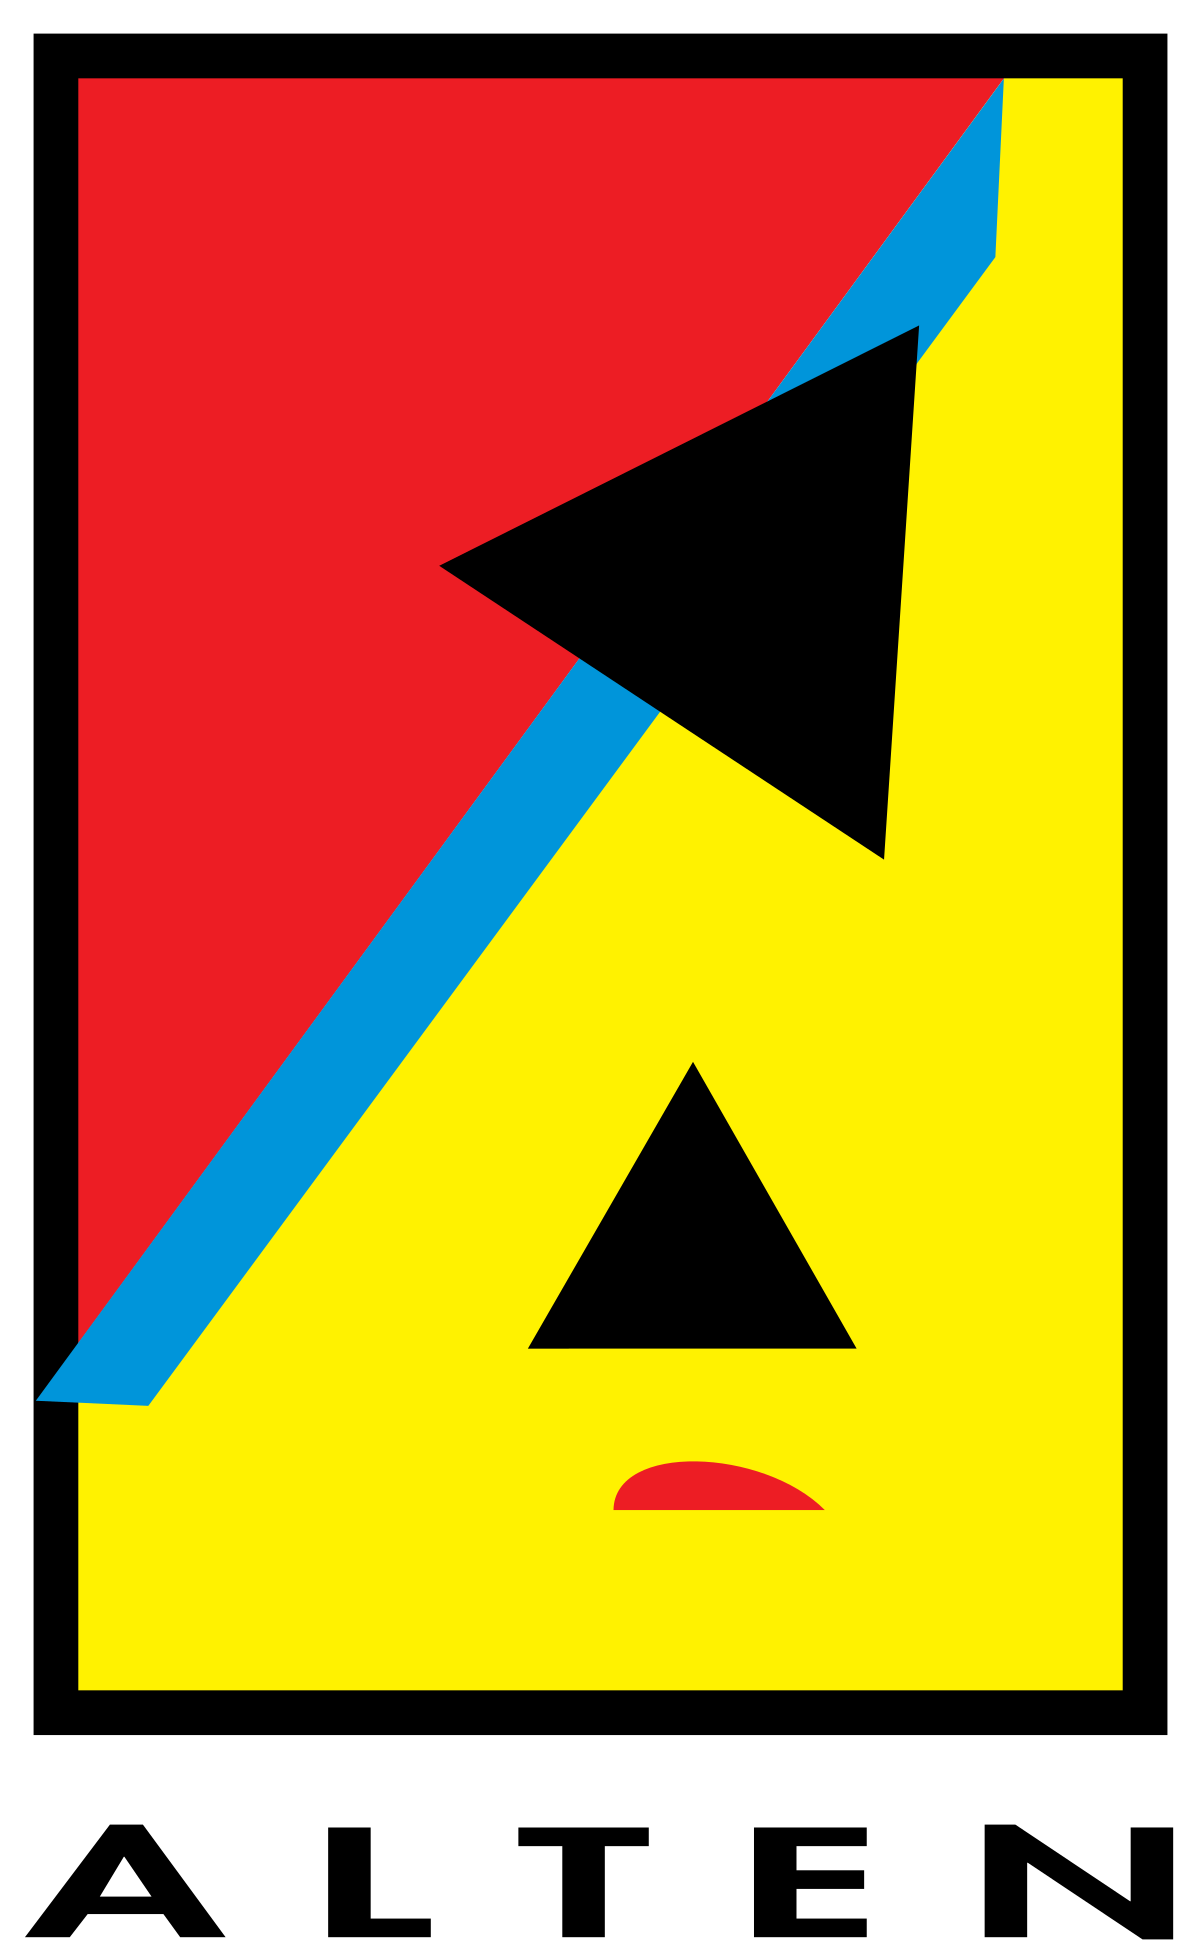
\includegraphics[scale=0.1]{alten}\end{center}
\end{figure}
\maketitle

%\section*{Voorwoord}
%\addcontentsline{toc}{section}{\protect\numberline{}Voorwoord}
%\pagebreak

\tableofcontents
\clearpage
%\section*{Begrippenlijst}

% Please add the following required packages to your document preamble:
% \usepackage[table,xcdraw]{xcolor}
% If you use beamer only pass "xcolor=table" option, i.e. \documentclass[xcolor=table]{beamer}
%\begin{table}[H]
%\centering

%\label{begrippen}
%\begin{tabular}{|l|l|}
%\hline
%\rowcolor[HTML]{C0C0C0}
%Term        & Omschrijving                                                         \\ \hline
%term        & Omschrijving                                                      	\\ \hline

%\end{tabular}
%\caption{Begrippenlijst}
%\end{table}

%\clearpage

%\section*{Samenvatting}
%\addcontentsline{toc}{section}{\protect\numberline{}Samenvatting}
%\pagebreak

\chapter*{Samenvatting}

Optioneel een samenvatting van het onderzoek. Hier kunnen anderen snel inzicht krijgen in wat jij hebt onderzocht en wat je conclusie is.
\begin{itemize}
	\item Kunnen derden snel inzicht krijgen in jouw onderzoek?
	\item Staat de conclusie erin vermeld?
\end{itemize}
\hrule

\chapter{Inleiding}
\label{chapter:inleiding}


De inleiding beschrijft:
\begin{itemize}
\item Waarvoor het onderzoek gedaan wordt;
\item Beschrijf waarom het onderzoek nu wordt uitgevoerd;
\item Het doel van het onderzoek.
\end{itemize}
\hrule

Het volgende onderzoek rapport wordt uitgevoerd ten behoeve van de het afstudeerproject van Maurice Berentsen, Hogeschool van Arnhem en Nijmegen.

Het doel van dit onderzoek is het zetten van de eerste stap in de ontwikkeling van het
dronenetwerk. De eerste stap is ontwikkelen van een netwerkmodule voor het onderling
verbinden van drones. Het is van belang dat het meshnetwerk van de drones snel kan
reageren op uitval van netwerkpunten.


\chapter{Hoofd- en deelvragen}
In dit hoofdstuk worden de hoofd- en deelvragen genoemd en onderbouwd.
Er wordt een scope bepaalt met wat er onderzocht wordt en dus ook wat niet.
Vervolgens wordt de onderzoeksmethode toegelicht en beargumenteerd.
Tenslotte wordt de invloed van het onderzoek op het afstudeerproject beschreven.

\section{Hoofdvraag}
Het doel van dit onderzoeksrapport is het beantwoorden van de volgende opgesteld hoofdvraag:
\begin{quotation}
\textit{Hoe kunnen een netwerkmodules een groep van ongeveer 100 drones voorzien van een onderling meshnetwerk die snel reageert op uitval van netwerkpunten?}	
\end{quotation}
Doordat de uitvoerende student van dit onderzoek niet beschikt over een certificaat om met drones te mogen vliegen behoudt dit onderzoek zich tot een simulatie.
Van de netwerkmodule wordt wel een fysiek prototype ontwikkeld.

\section{Deelvragen}

Om de hoofdvraag te kunnen beantwoorden zijn er de volgende deelvragen opgesteld:

\begin{itemize}
	\item Welke simulatie software is geschikt om een netwerk van ongeveer 100 drones in na te bootsen?
	\item Wat is de grote van de payload die een netwerkmodule aangesloten op een drone moet versturen om nuttig te zijn voor het aansturingssysteem?
	\item Welke mesh netwerk hardware is geschikt voor het onderling verbinden van drones?
	\item Welke mesh netwerk techniek is geschikt voor de te gebruiken hardware?
	\item Hoe gedraagt een node uit het mesh netwerk zich bij slecht of geen bereik?
	\item Wat kan er toegevoegd worden aan de communicatie van de netwerkmodule om snel [TODO snel definiëren] achter uitval te komen?
	\item Wat is minimaal benodigd in een simulatie om abstracte drone te representeren?
\end{itemize}

\section{Onderzoeksmethode}
De onderzoeksmethodes volgen de structuur van de \textit{ICA methodenkaart} \cite{MethodenKaart}.
De methodenkaart is een onderzoek framework voor professionals in ICT en media.
Het ontwerp van het framework gaat uit van het idee van triangulatie.
Triangulatie is het combineren van verschillende theorieën, methoden of databronnen om zo tot betere antwoorden te komen op je onderzoeksvragen \cite{ICAoates}. 
Door het definiëren van zo geheten werkplaatsen en hun samenhang geeft het de onderzoeker een set van methoden en technieken. 
De vijf verschillende werkplaatsen binnen het framework zijn: \textit{lab, veld, showroom, bieb en werkplaats}.

\begin{figure}[H]
	\begin{center}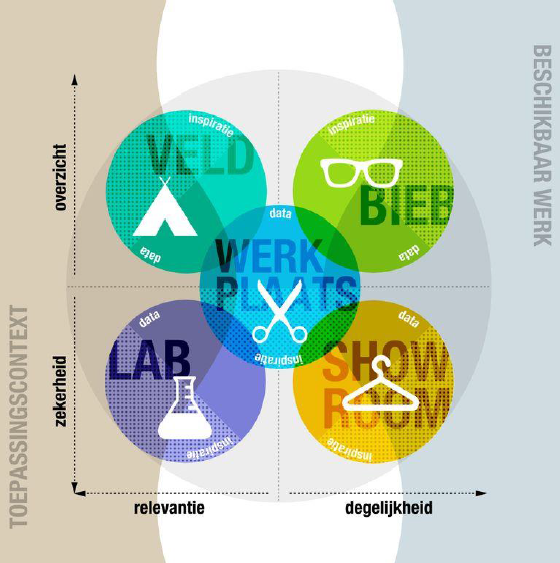
\includegraphics[width=0.5\linewidth]{Methodenkaart}\end{center}
	\caption{De vijf werkplaatsen binnen het framework en hun systematiek. Overgenomen uit \textit{De informatieprofessional 3.0}  van \protect\citeA{MethodenKaart}  }
	\label{fig:methodenkaart}
\end{figure}

\subsection{De gekozen onderzoeksmethodes}

De deelvragen gaan gedeeltelijk over keuzes van gebruik. 
Welke software en hardware is geschikt, is een vraag die veel naar voren komt.
Hieruit valt te concluderen dat de onderzoeker zich nog aan het oriënteren is.
"De onderzoeksruimte bieb bevat een verzameling methoden en technieken die dienen tot oriëntatie op beschikbaar werk."\cite{MethodenKaart}
Daarom wordt er gekozen om een bieb onderzoek uit te voren naar de deelvragen die gaan over geschiktheid.
Dit zodat de onderzoeker zich nog kan oriënteren naar het beschikbare aanbod en nog op nieuwe deelvragen kan komen. 

Lab onderzoek wordt pas later uitgevoerd omdat niet alle hardware voor handen is, maar ook omdat er niet genoeg tijd voor beschikbaar is.
\citeauthor{MethodenKaart} zegt het volgende over lab onderzoek: De onderzoeksruimte lab bevat methoden die geschikt zijn om de oplossing te toetsen aan een aspect van de toepassingscontext.
Daarom is het lab onderzoek geschikt voor het moment waarop de hardware beschikbaar is en de onderzoeker het gedrag hiervan exact in kaart wil brengen en wil bewijzen dat de gestelde eisen behaald worden.

\citeA{ICAoates} stelt dat een systeem bouwen 'bewijs' is dat een nieuw soort toepassing gebouwd kan worden. Als dit het doel is heeft het onderzoek waarschijnlijk hoofdzakelijk een werkplaats karakter, maar alle andere onderzoeksruimtes kunnen een rol spelen.
Gedurende het huidige onderzoek zal er door de onderzoeker software geschreven worden om bewijs te leveren dat een netwerkmodule een groep drones kan voorzien van een onderling netwerk.
Daarom past de werkplaats onderzoeksruimte goed bij dit onderzoek.


\section{Invloed op het project}



\chapter{Criteria}
\label{chapter:criteria}
%Maak hier een lijst met criteria aan de hand van de hoofd- en deelvragen.
%\begin{itemize}	
%\item Zijn de criteria duidelijk opgesteld?
%\item Waar moet de oplossing aan voldoen, staat dit erin?
%\end{itemize}
%\hrule

In \autoref{tab:criteria} worden codes gebruikt als naam voor de criteria, wat deze betekenen wordt eerst toegelicht:
\begin{itemize}
	\item ALG: Een algemene eis die in elke onderzoek meegenomen moet worden.
	\item SK: Een eis die gesteld worden in de keuze naar simulatie software.
	\item DR: Een eis voor de te gebruiken drone in de simulatie.
	\item PH: Eisen opgesteld aan de prototype hardware.
	\item PS: Eisen opgesteld aan de prototype software.
\end{itemize}

\begin{longtable}{|l|l|l|}
	\hline
	\rowcolor[HTML]{C0C0C0} 
	Naam & Beschrijving \\ \hline
	%\endfirsthead
	%
	\endhead
		\hypertarget{alg1}{ALG1}	&Is voorzien van API documentatie.        \\ \hline
		\hypertarget{alg2}{ALG2}	&Ondersteunt aansturing vanuit C++ .    \\ \hline
		\hypertarget{alg3}{ALG3}	&\begin{tabular}[c]{@{}l@{}}Heeft ondersteuning voor het Linux platform Ubuntu 18.04\end{tabular}        \\ \hline
		\hypertarget{alg4}{ALG4}	&Software is gratis in gebruik voor studenten        \\ \hline
		\hypertarget{sk1}{SK1}		&\begin{tabular}[c]{@{}l@{}}Heeft ondersteuning voor UAV (unmanned air vehicle) ook wel drone genoemd\end{tabular} \\ \hline
		\hypertarget{sk2}{SK2}		&\begin{tabular}[c]{@{}l@{}}Ondersteunt de simulatie van locatie bepaling sensoren zoals GPS.\end{tabular}        \\ \hline
		\hypertarget{sk3}{SK3}		&\begin{tabular}[c]{@{}l@{}}Heeft een kant en klare oplossing voor simulatie van externe krachten zoals wind.\end{tabular}        \\ \hline
		\hypertarget{sk4}{SK4}		& Heeft een ingebouwde pathfinding oplossing.        \\ \hline
		\hypertarget{sk5}{SK5}		& Ondersteunt ROS als middleware.        \\ \hline
		\hypertarget{sk6}{SK6}		& Ondersteunt de detectie van botsingen.        \\ \hline
		\hypertarget{sk7}{SK7}		& Ondersteunt de simulatie 100 drones tegelijk.        \\ \hline
		DR1		& De drone is een quadcopter.        \\ \hline
		DR2		& De drone is is voorzien van een API voor aansturing op basis van coördinaten.       \\ \hline
		DR3		& De API sluit aan op de middleware ROS melodic.        \\ \hline
		DR4		& De drone is bruikbaar binnen de gekozen simulatie software.        \\ \hline%TODO gekozen software toevoegen
		DR5		& De drone moet een kleine goedkope drone representeren.        \\ \hline
		\hypertarget{ph1}{PH1}		& Ondersteunt een bereik van minimaal 500 meter.  \\ \hline
		\hypertarget{ph2}{PH2}		& Ondersteunt het gebruik van grid networking om tot een mesh te kunnen komen.  \\ \hline
		\hypertarget{ph3}{PH3}		& Maakt gebruik van een openbare bandbreedte.\\ \hline
		\hypertarget{ph4}{PH4}		& Voorziet zichzelf van een draadloos netwerk en leunt dus niet op technieken zoals 4G\\ \hline
		\hypertarget{ph5}{PH5}		& Is een product ontwikkeld voor low energy toepassingen. \\ \hline
		PS1		& Ondersteunt een mesh netwerk van minimaal 100 nodes. \\ \hline
		PS2		& Het netwerk is zelf herstellend. \\ \hline
		PS3		& Ondersteunt het draaien op een raspberry pi of een ardunio (UNO of NANO). \\ \hline
		PS4		& Ondersteunt het versturen van zelfgemaakte berichten. \\ \hline
		
	\caption{Opgestelde criteria}
	\label{tab:criteria}
\end{longtable}

\chapter{Literatuur}


\section{Welke simulatie software is geschikt om een drone in na te bootsen?}
\label{sec:welkesim}
Voor het onderzoek wordt gebruik gemaakt van een simulatie omgeving.
Welke software wordt gebruik staat vastgesteld in deze paragraaf.
De keuze van software wordt bepaald door het uitvoeren van de bieb onderzoeksmethode. 
In de \autoref{tab:criteria} staan de criteria toegelicht waar de simulatie software aan moet voldoen.
Als hoofdcriteria wordt een lijst opgesteld met simulatoren die ondersteuning hebben voor ROS.
Vervolgens worden deze aan de hand van een kruistabel onderworpen aan de andere criteria.
Deze techniek is gebaseerd op de "Comparison Chart" van \cite{CMDmethod} uit de "\textit{CMD Methods Pack}"

De kandidaten zijn:
\begin{itemize}
	\item \href{https://www.energid.com/actin}{Actin} is een simulatie framework van het bedrijf Energid. Het is in staat om de beweging van verschillende robots gelijktijdig aan te sturen.
	\item \href{http://gazebosim.org/}{Gazebo} is een opensource robot simulatie framework bijzonder geschikt voor het simuleren van robotica in outdoor omgevingen door de uitgebreide Physics Engine Support.
	\item \href{http://www.coppeliarobotics.com/}{V-REP (Virtual Robot Experimentation Platform)} is een platform geschikt voor het snel bouwen van robot prototypes.
	\item \href{https://cyberbotics.com/}{Webots} is een open source-ontwikkelomgeving die wordt gebruikt voor het modelleren, programmeren en simuleren van mobiele robots.
	\item \href{http://openrave.org/}{OpenRAVE} biedt een ontwikkelomgeving voor het testen van motion planning algoritmes aan de hand van simulaties.
\end{itemize}

\begin{table}[H]
	\centering
	\begin{tabular}{l|*{10}r}
		%\backslashbox{Input}{Output} & int8\_t & int16\_t & int32\_t & uint8\_t & uint16\_t & uint32\_t \\
		\diagbox[width=2.7cm, height=2.4cm]{\raisebox{5pt}{\hspace*{0.25cm}Simulator}}{\raisebox{-1.27cm}{\rotatebox{90}{Eis}}} & \raisebox{-0.25cm}{\rotatebox{90}{\hyperlink{alg1}{ALG1}}} & \raisebox{-0.25cm}{\rotatebox{90}{\hyperlink{alg2}{ALG2}}} & \raisebox{-0.25cm}{\rotatebox{90}{\hyperlink{alg3}{ALG3}}} & \raisebox{-0.25cm}{\rotatebox{90}{\hyperlink{alg4}{ALG4}}} &
		\raisebox{-0.25cm}{\rotatebox{90}{\hyperlink{sk1}{SK1}}} & \raisebox{-0.25cm}{\rotatebox{90}{\hyperlink{sk2}{SK2}}} &
		\raisebox{-0.25cm}{\rotatebox{90}{\hyperlink{sk3}{SK3}}} & \raisebox{-0.25cm}{\rotatebox{90}{\hyperlink{sk4}{SK4}}} &
		\raisebox{-0.25cm}{\rotatebox{90}{\hyperlink{sk5}{SK5}}} & \raisebox{-0.25cm}{\rotatebox{90}{\hyperlink{sk6}{SK6}}} \\
		\midrule\\
		\hspace*{0.25cm}Actin 	& \checkmark & \checkmark 	& \checkmark & x 		  & \checkmark & x 			& \checkmark & x 		  &\checkmark & \checkmark	\\ \\
		\hspace*{0.25cm}Gazebo 	& \checkmark & \checkmark 	& \checkmark & \checkmark & \checkmark & \checkmark & \checkmark & \checkmark &\checkmark & \checkmark	\\ \\
		\hspace*{0.25cm}V-REP 	& \checkmark & x 			& \checkmark & \checkmark & \checkmark & \checkmark & \checkmark & \checkmark &\checkmark & x	\\ \\
		\hspace*{0.25cm}Webots 	& \checkmark & \checkmark 	& \checkmark & \checkmark & \checkmark & \checkmark & \checkmark & \checkmark &\checkmark & \checkmark 	\\ \\
		\hspace*{0.25cm}OpenRAVE& \checkmark & \checkmark	& \checkmark & \checkmark & x 		   & \checkmark & \checkmark & \checkmark &\checkmark & x 	\\ \\
		\bottomrule
	\end{tabular}%
	\caption{Kruistabel simulatiekeuze}
	\label{tab:kruissimkeuze}%
\end{table}%

In de \autoref{tab:kruissimkeuze} komt de simulatie software van Gazebo en Webots naar voren als enige simulatoren die voldoen aan alle gestelde eisen.
Het is nu zaak om te uit te zoeken welke van de twee het meest geschikt is voor het uitvoeren van dit onderzoek.

\subsection{Gazebo of Webots?}
In januari 2018 hebben \citeauthor{RobotCompare} een publicatie geschreven waarin zij drie simulatoren vergelijken in het aanbod van features en performance. 
Zij hebben een vergelijking gedaan tussen V-REP, Gazebo en ARGoS. 
ARGoS is niet meegenomen in de overweging omdat het geen ondersteuning heeft voor ROS.

In de conclusie van de publicatie komt Webots als het meest gebruiksvriendelijk naar voren in het gebruik en is in het bezit van de meeste features.
Het grote nadeel van Webots is dat het veel kracht vraagt van de computer waardoor het niet geschikt is voor de simulatie van veel drones tegelijk.

Daarmee komt de keuze uit op Gazebo. 
De resultaten in de publicatie van \citeA{RobotCompare} tonen aan dat de software in staat is om veel drones tegelijk aan te kunnen sturen.
\citeA{RobotCompare} geven als nadeel aan Gazebo dat de software niet in staat is om 3d meshes te manipuleren, de user interface niet innovatief is en Gazebo soms problemen met dependencies door de verschillende versies van ROS.
Dit laatste brengt een risico met zich mee voor het onderzoek daarom is het ook zaak dat dit als criteria meegenomen word in de deelvraag van \autoref{sec:dronekeuze} \nameref{sec:dronekeuze}. 

\subsection{Conclusie}
Voor het onderzoek wordt Gazebo gebruikt omdat het voldoet aan de gestelde \nameref{chapter:criteria}.
De meest recente versie van Gazebo, die niet meer beta is op 19 februari 2019, is Gazebo 9.
Deze versie vereist het gebruik van ROS Melodic volgens haar eigen website  (\href{http://gazebosim.org/tutorials?tut=ros_wrapper_versions}{zie link}).

\section{Wat is de grootte van de payload die een netwerkmodule aangesloten op een drone moet versturen om nuttig te zijn voor het aansturingssysteem?}

De payload is het gedeelte van een bericht die vrij is naar de gebruiker om invulling te geven.
De maximale grote van een payload verschilt per protocol.
Om een keuze te kunnen maken waar de hardware en het bijhorende protocol aan moet voldoen is het dus zaak om eerst te weten hoe groot deze vrije payload ruimte moet zijn.

Het doel van de berichten is om ze zo kort als mogelijk samen te stellen. 
Daarom is het belangrijk om de structuur van de berichten zo klein mogelijk te houden.
Om deze reden wordt niet gekeken naar een tekstuele serialisatie mogelijkheden zoals XML, YAML, JSON maar naar binaire mogelijkheden omdat deze veel efficienter zijn \cite{binary}.

\subsection{Binaire serialisatie voor het samenstellen van berichten} 

"Binary Serialization is converting the object in binary format and being able to store it in a storage medium"\cite{binary}. 
Het binair samenstellen van informatie is een efficiënte manier omdat de data met een minimale overhead wordt samengesteld \cite{binaryMessaging}
Het nadeel die deze wijze met zich meebrengt is dat het resultaat van het bericht niet meer makkelijk leesbaar is voor mensen.
Voor dit project ligt daar geen focus op dus is dit nadeel te verwaarlozen.

\citeA{binaryMessaging} hebben onderzoek gedaan naar een efficiënte manier naar de inzet van binaire berichten te vervanging van tekstuele serialisatie.
Hoewel dat in het huidige onderzoek niet het geval is kan er wel geleerd worden van de manier van bericht gebruik.
\citeA{binaryMessaging} tonen in hun onderzoek aan dat berichten vaak een herhalende structuur hebben en dat dit een onnodige overhead creëert in de berichten.
Een voorbeeld maken \citeA{binaryMessaging} zichtbaar in \autoref{fig:jsonxml} waarover zij het volgende zeggen: "While JSON  compared  with  XML,  eliminated  parameter  name redundancy, it keeps repeating (red box) the definition of each field  for  each  serialized  element  (green  box)". 
\begin{figure}[H]
	\begin{center}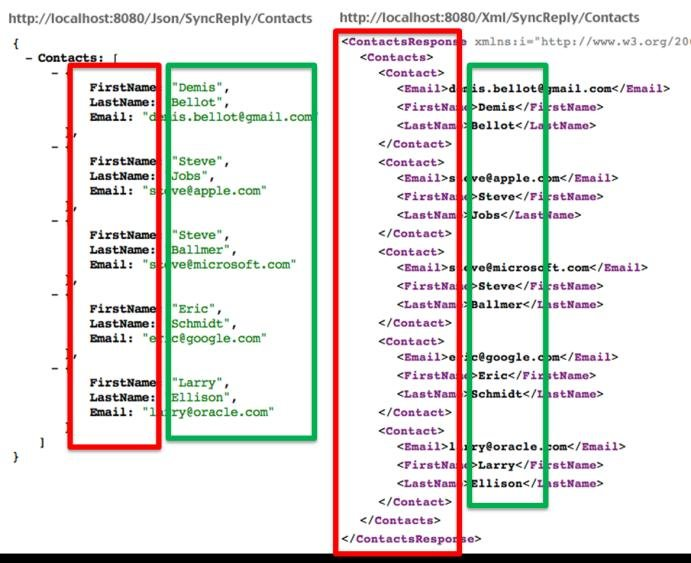
\includegraphics[width=0.5\linewidth]{JSONandXML.jpeg}\end{center}
	\caption{JSON and XML messages. Overgenomen uit \textit{International Journal of Computer Applications}  van \protect\citeA{binaryMessaging}  }
	\label{fig:jsonxml}
\end{figure}

Wat zij hebben gedaan om dit op te lossen is het apart versturen van de parameternamen zodat deze in de opvolgende berichten van dat type niet meer nodig is.
Het systeem die bedacht is geeft een enorme flexibiliteit omdat er van te voren nog geen bericht types bekend hoeven te zijn.
Deze flexibiliteit is alleen niet van toepassing op het doel van dit project, daarom kan de student in zijn software al van te voren berichttypes samenstellen waardoor er de overhead nog kleiner gemaakt wordt.
Voor nu wordt er vanuit gegaan dat 1 byte genoeg zal zijn omdat de communicatiesoftware van de netwerkmodule niet meer dan 256 ($2^{8}$) berichtentypes hoeft te ondersteunen.
Mocht het blijken dat dit toch niet genoeg is kan er er een byte toegevoegd worden waardoor er 65536 ($2^{16}$) types mogelijk zouden zijn.
Daarnaast moet een bericht om nuttig te zijn voor het netwerk altijd aan een apparaat gekoppeld kunnen worden.
De opdracht gaat over een netwerk van ongeveer 100 drones wat ruim past in een byte
Daarom wordt er gekozen om een byte te gebruiken wat 255 unieke ID's mogelijk zou maken. 
Hiermee komt het eerste deel van het bericht dus al tot stand het telt nu minimaal 2 bytes.

\begin{table}[H]
	\centering
	\begin{tabular}{|l|l|l|}
		\hline
		\rowcolor[HTML]{C0C0C0} 
		ID & Berichttype & overig \\ \hline
		00 tot FF   & 00 tot FF       & ?      \\ \hline
	\end{tabular}
	\caption{Berichtsamenstelling met type aanduiding}
	\label{tab:serialstart}
\end{table}

\subsection{Wat is nuttige informatie die in een bericht kan staan voor of van een aansturingssysteem?}
\label{sub:watisnuttigeinformatie}
Hoewel er nog niet bekend is welk type netwerk er gebruikt gaat worden is het al wel bekend dat dit een low power long range netwerk zal zijn om aan de requirements te voldoen.
Een gedeelde eigenschap van zulke netwerken is de lage bandbreedte waardoor ze niet geschikt zijn voor realtime applicaties.
Deze kennis kan toegepast worden op de informatie die de drones met hun netwerkmodules bij zich dragen. 
Informatie zoals snelheid en richting heeft geen prioriteit om verstuurd te worden omdat deze niet relevant is voor het aansturingssysteem aangezien hier geen beslissingen op gebaseerd kunnen worden.
Wat wel van belang is voor het aansturingssysteem is informatie als waar bevindt een netwerkmodule zich op welk moment in tijd.
Daarnaast kan informatie zoals de status van de batterij en de sterkte van de verbinding van belang zijn voor het systeem omdat deze informatie gebruikt kan worden om preventieve beslissingen te nemen in het onderhoud van het netwerk.

Een bericht die het aansturingssysteem tenminste zal verzenden zal het commando zijn om een drone naar een coordinaat te sturen.
Daarnaast zal er een bericht moeten komen waarmee het systeem de status van het netwerk kan controleren, wat voor bericht dit zal zijn is nog niet bekend.


\subsection{Wat is de grootte van een bericht voor de locatie bepaling van drones?}
\label{sub:locatie}
De huidige locatie is essentiële administratie voor de verdeling van de drones.
Omdat de drones zich kunnen verplaatsen is naast de locatie ook het tijdstip waarop het bericht verstuurd wordt van belang.

\subsubsection*{Coördinaat vanuit de informatie van de GPS module}
Een positie van een locatie wordt aangeduid door coördinaten te gebruiken.
Deze worden bepaald door het gebruik van een GPS module aan boord van het systeem.
GPS modules gebruiken triangulatie van satellietsignalen om hun positie te bepalen.  

Een coördinaat is opgebouwd door de aarde te verdelen in graden over de assen latitude (horizontaal) en longitude (verticaal).
Een coördinaat loopt van -180 tot 180 graden.
De aarde heeft een omtrek van 40.07.5161,2 meter gedeeld door 360 graden levert dit per graad een stap op van 111,32 kilometer. 
Het volgende programma laat zien dat een float gebruikt kan worden in dit geval voor een accuraatheid van 5 cijfers achter het decimaal.

\begin{lstlisting}
#include <stdio.h>

float exampleFloatPositive = 179.1234567890;
float exampleFloatNegative = -179.1234567890;

int main( int argc, const char* argv[] )
{
	printf( "postive  float =  %f\n", exampleFloatPositive );
	printf( "negative float =  %f\n", exampleFloatNegative );
}
\end{lstlisting}
 
Door een coördinaat te gebruiken van 5 cijfers achter het decimaal kan een plek op aarde met een precisie van ongeveer 1,10 meter nauwkeurig aangeven worden.
Het is gebruik hiervan is realistisch omdat met alleen realtime GPS data de accuraatheid ongeveer 4 meter is \cite{GPSaccu}.
Er wordt per as een float gebruikt dit houdt in dat minimaal 8 bytes nodig zijn voor een coördinaat.
Dit is 4 bytes per float en exclusief de separator. 

\subsubsection*{Hoogte van de drone}
\citeA{GPSheight} hebben onderzoek gedaan naar de accuraatheid van de hoogtebepaling bij drones. 
Uit dit onderzoek is gebleken dat een continue vliegende drone een accuraatheid heeft van ongeveer twee meter.
Hieruit is te halen dat het geen zin heeft om op centimeter niveau de hoogte van een drone aan te geven.
Op het moment dat er een signed integer van 16 bits gebruikt zou worden kan er een afstand van 32.767 meter zowel boven als onder zeeniveau verstuurd worden.
Het is een realistische waarde om te gebruiken aangezien de grootste hoogte die gebruik kan worden dan 32 kilometer is.
Deze hoogte is al ver in de stratosfeer en zelfs al boven het niveau die een weerballon haalt. 
De keuze om een signed integer te gebruiken is om ondersteuning te bieden aan plekken onder het zeeniveau waarvan Nederland een groot voorbeeld is.

Voor de hoogte moeten 2 bytes gereserveerd worden. 

\subsubsection*{Tijd vanuit de GPS module}

De drone maakt al gebruik van de GPS module voor de positiebepaling.
In de berichten die de GPS module ontvangt van de satellieten wordt ook de tijd meegestuurd.
Deze tijd is volgens \cite{GPSaccu} in 95 procent van de gevallen accuraat tot 40 Nano seconden. 
In het geval van het drone netwerk is dit veilig te gebruiken als bron voor tijd.
De tijd zal aangegeven worden in het unix time format zodat deze meteen de datum met zich draagt.
Unix time maakt gebruik van 32 bits formaat, er is gekozen voor een unsigned variant aangezien er geen interesse is naar data voor 1 januari 1970 ook wel epoch genoemd.

Voor de tijd en datum worden 4 bytes gereserveerd.

\subsubsection*{Conclusie}  

De bovenstaande sub paragrafen kunnen samengesteld worden tot een bericht waarin alle informatie zit die nodig is om te bepalen waar een drone zich op een moment bevindt.
Een systeem kan met dit bericht in ieder geval elke drone afzonderlijk in kaart brengen.

\begin{table}[H]
	\centering
\begin{tabular}{l|l|l|l|l|l|l|}
	\cline{2-7}
	& \cellcolor[HTML]{C0C0C0}ID & \cellcolor[HTML]{C0C0C0}\begin{tabular}[c]{@{}l@{}}Bericht \\ type\end{tabular} & \cellcolor[HTML]{C0C0C0}latitude & \cellcolor[HTML]{C0C0C0}longitude & \cellcolor[HTML]{C0C0C0}hoogte & \cellcolor[HTML]{C0C0C0}tijd \\ \hline
	\multicolumn{1}{|l|}{\cellcolor[HTML]{C0C0C0}\begin{tabular}[c]{@{}l@{}}Aantal\\ Bytes\end{tabular}} & 1                          & 1                                                                               & 4                                & 4                                 & 2                              & 4                            \\ \hline
\end{tabular}
 \caption{Locatie bericht in bytes}
\label{tab:locatiebericht} 
\end{table}
In \ref{tab:locatiebericht} is het aantal bytes te zien benodigd voor een locatie bericht.
Concluderend wordt voor dit bericht een grootte van minimaal 16 bytes gebruikt.
 
\subsection{Wat is de grootte van een bericht waarin een netwerkmodule zijn verbinding met anderen aangeeft?}

Een van de wensen van de Alten is het in kaart brengen van de onderlinge verbindingen van de modules in het drone netwerk. 
Als voorbeeld hoe dit eruit kan zien is de schets afkomstig van de casus uit het plan van aanpak toegevoegd als bijlage te vinden in \autoref{app:schetsNetwerk}.
De informatie van de locatie van de netwerkpunten zijn al bekend door het gebruik van het bericht in \autoref{sub:locatie}
Wat overblijft als onbekende informatie is de onderlinge verbinding.

In het netwerk kunnen twee rollen verdeeld worden.
De rol van zender aan het device die informatie wil versturen naar het basis station.
Of de rol van ontvanger aan het device die de informatie van zender ontvangt.
Een device die beide rollen kan aannemen wordt een transceiver genoemd.
Als werkbaar voorbeeld wordt het netwerk uit de \nameref{app:schetsNetwerk} gebruikt.
De ontvangers en zenders zijn verdeelt in \autoref{tab:ontvangerzender}.

\begin{table}[H]
\centering
\begin{tabular}{
		>{\columncolor[HTML]{C0C0C0}}r |c|c|c|c|c|c|c|c|c|c|c|c}
	Ontvanger & BS   & 9   & 7 & 5 & 3 & 2 & 8 & 6 & 11    & 13 & 12 & 14       \\ \hline
	Zender    & 9,11 & 7,8 & 5 & 3 & 2 & 1 & 6 & 4 & 13,10 & 12 & 14 & 15,16,17
\end{tabular}
	\caption{De ontvangers en zenders uit de casus}
	\label{tab:ontvangerzender}
\end{table} 

\subsubsection*{Topologie met PlantUML}  
Om snel aan te kunnen tonen dat er weinig informatie nodig is om een topologie op te stellen gebruikt de student PlantUML.
Hiermee wordt aangetoond dat een bericht die de ontvanger aanmaakt zodra een zender zich bij hem aanmeld waar in staat wie de zender is genoeg is voor een topologie.
De keuze om de verantwoording bij de ontvanger neer te leggen is omdat een zender niet bij elke soort netwerk weet wie de ontvanger is.
De uitwerking hiervan is zichtbaar in \autoref{fig:toplogienetwerkuml}

\begin{figure}[H]
	\begin{center}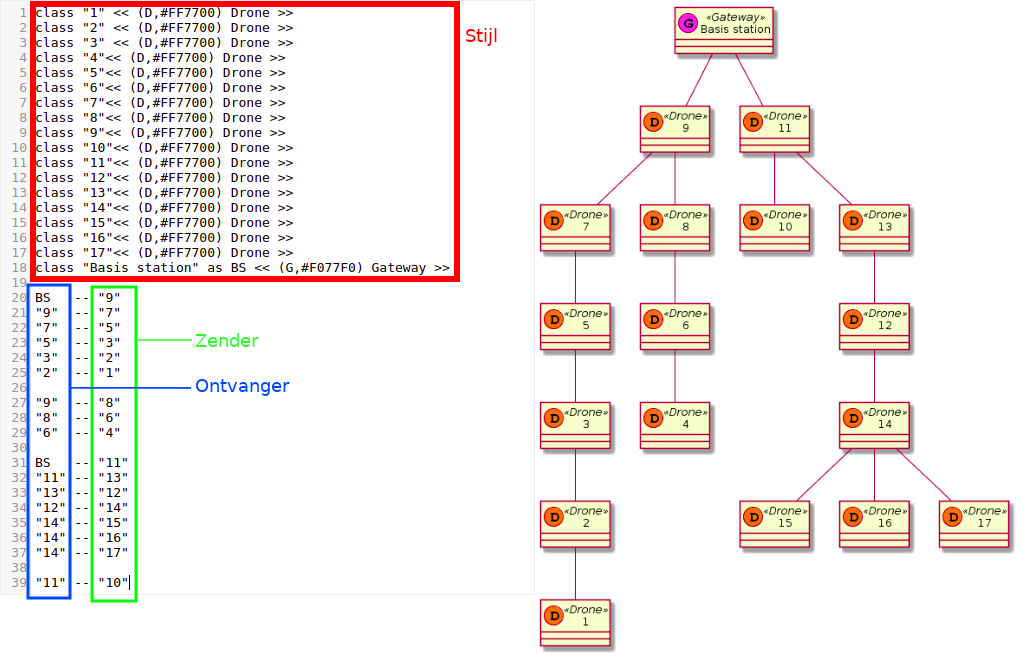
\includegraphics[width=\linewidth]{zenderontvangertopo}\end{center}
	\caption{Topologie van het casusnetwerk door middel van PlantUML}
	\label{fig:toplogienetwerkuml}
\end{figure}


\subsubsection*{Conclusie}  
Het ID van de ontvanger zit al in het bericht aangezien deze de opsteller van het bericht is.
Dit houdt in dat enkel een ID toegevoegd hoeft te worden van de aangemelde zender.
De byte grootte van de ID's is al bekend deze telt namelijk 1 byte.
Daarmee zou het bericht het volgende format krijgen te zien in \autoref{tab:topologiemessage}

\begin{table}[H]
	\centering
\begin{tabular}{l|l|l|l|}
	\cline{2-4}
	& \cellcolor[HTML]{C0C0C0}ID & \cellcolor[HTML]{C0C0C0}\begin{tabular}[c]{@{}l@{}}Bericht \\ type\end{tabular} & \cellcolor[HTML]{C0C0C0}ZenderID  \\ \hline
	\multicolumn{1}{|l|}{\cellcolor[HTML]{C0C0C0}\begin{tabular}[c]{@{}l@{}}			Aantal\\ Bytes\end{tabular}} & 1   & 1  & 1  \\ \hline
\end{tabular}
	\caption{Berichtsamenstelling aanmelding zender voor topologie}
	\label{tab:topologiemessage}
\end{table}
Dit houdt in dat dit bericht een totaal van 3 bytes telt.

\subsection{Conclusie}
\label{sec:payloadconclusie}

In deze paragraaf wordt antwoord gegeven op de vraag: Wat is de grootte van de payload die een netwerkmodule aangesloten op een drone moet versturen om nuttig te zijn voor het aansturingssysteem?
Er is gekeken hoe het bericht opgesteld moet worden en naar de inhoud van twee verschillende berichten die relevant zijn voor het aansturingssysteem.
Het grootste bericht van deze twee was het bericht waar in staat op welke positie de netwerkmodule zich bevindt.
Dit bericht telt 17 bytes en is een bericht die informatie bevat van vier verschillende waardes.
Hoewel er meer berichten zullen bestaan in het netwerk is het onaannemelijk dat deze groter zullen zijn dan deze 17 bytes.
Om toch ruimte te houden voor extra informatie in een bericht voor bijvoorbeeld data verificatie worden er 4 bytes toegevoegd aan het maximum. 
Dit zou voldoende ruimte moeten geven doordat er één 32 bits waarde of twee 16 bits waardes toegevoegd kunnen worden.

Daarmee is de conclusie dat de maximale grootte 21 byte is voor een bericht om nuttig te zijn voor een aansturingssysteem.

\section{Welke mesh netwerk hardware is geschikt voor het onderling verbinden van drones?}
\label{sec:meshnetwerkkeuze}

Om een onderling netwerk op te bouwen is hardware nodig. 
Deze hardware moet voldoen aan de gestelde \nameref{chapter:criteria} zodat het geschikt is voor een drone netwerk.
In \autoref{sec:payloadconclusie} is vastgesteld dat de payload berichten van 21 byte moet kunnen bevatten.
Criteria \hyperlink{ph1}{PH1} eist dat het bereik van de modules minimaal 500 meter is.
Vervolgens stelt criteria \hyperlink{ph5}{PH5} stelt dat het netwerk zuinig in gebruik moet zijn. 
\subsection{Wat is een meshnetwerk?}
\label{sec:meshnetwerkkeuze:watismesh}
Een meshnetwerk is een term die gebruikt wordt voor een topologie techniek in netwerken.
Om een voorbeeld beter toe te kunnen lichten worden eerst de tegenhangers besproken de ster en boom topologie.

Een doorsnee huishouden maakt zeer waarschijnlijk gebruik van een ster topologie.
Er staat een modem bij de aansluiting in het huis die een Wifi signaal uitzendt waar vervolgens alle mobiele apparaten mee verbinden en vaak nog een fysieke poorten aanbiedt voor een bekabelde verbinding.
Dat levert een topologie op zichtbaar in \autoref{fig:toplogiester}

\begin{figure}[H]
	\begin{center}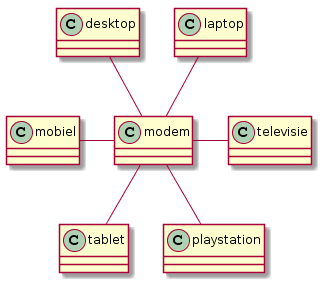
\includegraphics[width=.4\linewidth]{sterTopo}\end{center}
	\caption{Topologie van ster netwerk}
	\label{fig:toplogiester}
\end{figure}

In de meeste huishoudens volstaat dit aangezien de router bereikbaar is vanaf elk punt in het huis.
Op het moment dat dit niet zo is het gangbaar om uit te wijken tot een boom topologie door een of meerdere routers toe te voegen in het netwerk.
Vertaalt naar een topologie zou dit er als \autoref{fig:toplogieboom} uitzien.

\begin{figure}[H]
	\begin{center}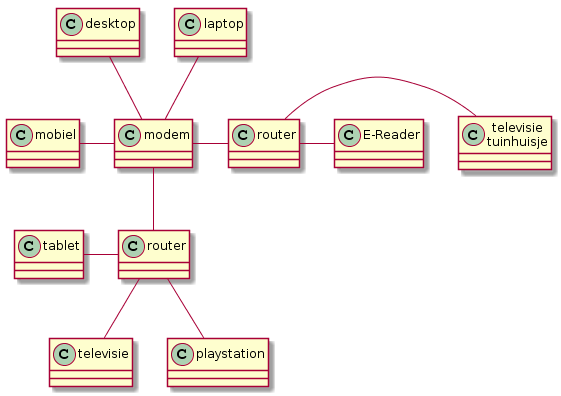
\includegraphics[width=.5\linewidth]{treeTopo}\end{center}
	\caption{Topologie van boom netwerk}
	\label{fig:toplogieboom}
\end{figure}

Een probleem wat uit deze twee voorbeelden duidelijk wordt is de grens van het bereik. 
Deze is namelijk alleen uit te breiden in door het toevoegen van extra netwerkpunten.
De mesh netwerk techniek is een oplossing voor dit probleem.
In een meshnetwerk zijn de apparaten in staat om direct met elkaar te verbinden. 
Zo is elk apparaat in het netwerk direct een uitbreiding in het bereik van het netwerk doordat het informatie kan doorgeven.

Er zitten aan een meshnetwerk ook nadelen.
Omdat er nu meerdere routes van en naar een apparaat zijn komt er een extra protocol bij kijken welke route genomen moet worden wat extra complexiteit toevoegt.
Daarnaast zal het draadloze verkeer verhoogt worden waardoor uiteindelijk apparaten elkaar zullen verstoren.
Tenslotte voegt het ook een afhankelijkheid toe omdat bijvoorbeeld de televisie in het tuinhuisje de laptop in de keuken gebruikt als stap naar het modem.

\begin{figure}[H]
	\begin{center}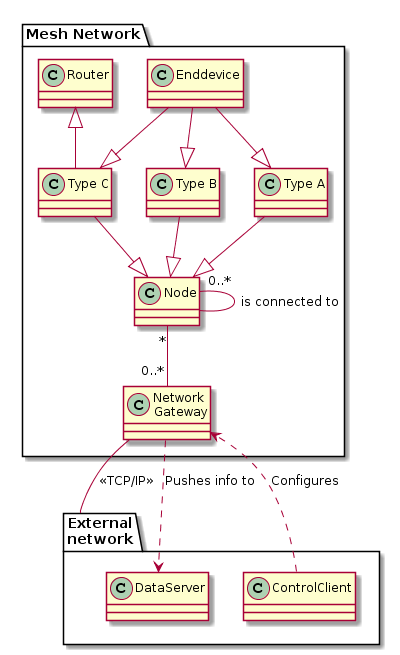
\includegraphics[width=.3\linewidth]{meshclass}\end{center}
	\caption{Verbanden tussen de rollen in een mesh netwerk}
	\label{fig:meshrol}
\end{figure}

In een meshnetwerk zijn er twee rollen te verdelen \cite{compNRF}.
Er is de rol van gateway waarmee het netwerk verbonden wordt naar een extern punt. 
En er is de rol van node welke in staat is om met een gateway te verbinden of met een andere node.

Een node is vervolgens weer te verdelen in drie types, de namen die hier aan gegeven worden verschillen per aanbieder voor het gemak worden die van LoRa gebruikt.
In LoRa wordt gesproken over type A, B en C waarbij elke type gericht is op een verschillende visie van stroomconsumptie \cite{LoraLimit}.

\begin{itemize}
	\item \textbf{Type A} is de energiezuinigste variant doordat het alleen online komt op het moment dat het data moet versturen.
Het grote nadeel van dat het communiceren naar dit type onmogelijk is en het dus ook niet bijdraagt het uitbreiden van het netwerk.
	\item \textbf{Type B} is een variant van type A welke na het zenden van een bericht enige tijd online blijft om een berichten te kunnen ontvangen. 
Een voordeel is dat deze dus wel op afstand aan te sturen is maar nog steeds is deze alleen een gebruiker van het netwerk.
	\item \textbf{Type C} is de minst zuinige variant van de nodes doordat hij altijd aan staat.
Het nadeel is dus dat deze het meest stroom verbruikt daarin tegen kan deze node wel de belangrijke rol krijgen van router en biedt vergroot daarmee het mesh netwerk.
\end{itemize}

In het geval van de opdracht wordt alleen gekeken naar type C nodes omdat er interesse is naar de dynamische plaatsing van dit type.





\subsection{LPWAN LoRa}
Deze twee eisen zijn een logische stap om een verdieping uit te voeren in low-power wide-area network (LPWAN) netwerken.

In de publicatie van \cite{LoraConnect} wordt het LoRaWAN netwerk onderzocht.
Ook worden daar de grootste concurrenten van het LoRaWAN netwerk benoemd namelijk \href{https://www.sigfox.com/en}{SigFox} en Narrowband IoT (NB-IoT).
Ondanks het feit dat deze protocollen niet interessant zijn voor het project omdat ze in de verkeerde OSI-laag vallen namelijk de netwerklaag is het wel interessant om te kijken welke techniek deze gebruiken.
NB-IoT valt direct af als interesse doordat het gebruikt maakt van mobiele communicatie en dus niet zou voldoen aan criteria \hyperlink{ph4}{PH4}.
Daarna valt SiGFox ook af simpelweg omdat het gebruik maar beperkt openbaar is gemaakt waardoor het niet geschikt is om een meshnetwerk mee te bouwen. 

Dan blijft uit deze publicatie het LoRaWAN netwerk over. 
Deze is gebasseerd op de LoRa fysieke laag (PHY)\cite{LoRAMOD} implementatie om de communicatie af te handelen.
LoRaWAN is een netwerkstandaard opgezet voor telecom providers om het mogelijk te maken netwerken op te zetten voor communicatie over afstanden tot 15km.
Alleen het LoRaWAN maakt gebruikt van een ster topologie doordat nodes maar 1 hop kunnen maken naar een gateway van het netwerk.
Een andere nadeel die het LoRa netwerk heeft is dat ondanks de grote afstand die het kan afleggen door de spreidingsfactor te vergroten en de gevoeligheid van de ontvanger te verhogen dit ten koste gaat van de snelheid van de datadoorvoer.
\citeA{LoraMesh} hebben in onderzoek gedaan naar de mogelijk om het LoRa PHY netwerk te gebruiken als mesh netwerk en ook aangetoond dat dit werkt.
Het doel van hun onderzoek was om door middel van mesh technieken LoRa geschikter te maken voor verstedelijkt gebied zonder het toevoegen van extra gateways. 
Een nadeel wat ze beschrijven in de conclusie is het aantal nodes wat ze kunnen verwerken verkleind wordt.
Dit komt door de degradatie van timing prestaties waarin ze stellen dat periode $p$ die een bericht nodig heeft om verstuurd te worden naar de gateway de volgende regel volgt ($p = 2h\cdot t$) waarbij $h$ het aantal hops is die het bericht maakt en $t$ de frametijd. Om de frametijd te berekenen geldt het volgende: $frametijd = \frac{framelengte}{bitsnelheid}$. 
Voordeel van het gebruik die een mesh kan hebben ten opzichte van een ster netwerk is dat het een hogere bitsnelheid kan behouden omdat er kleinere afstanden overbrugt hoeven te worden waardoor de frametijd alsnog klein kan blijven.
Een voorwaarde van het gebruik van dit netwerk is dus wel dat de framelengte klein moet zijn waardoor het niet geschikt is voor het verwerken van grote berichten zoals afbeeldingen video of andere grote bestanden.

\subsubsection*{LPWAN LoRa samengevat}
Als er gekeken wordt naar LPWAN oplossingen is LoRa PHY de enige noemenswaardige oplossing voor dit project.
\citeA{LoraMesh} hebben al aangetoond dat een mesh netwerk op bais van LoRa mogelijk is waardoor het risico afneemt in de haalbaarheid van dit onderzoek.
Een voordeel van dit netwerk is de afstand die de netwerkmodules van elkaar kunnen staan die met deze techniek kan oplopen tot meer dan 10 kilometer afhankelijk van de hoeveelheid en frequentie van de data die verstuurd moet worden.
Een ander voordeel van deze techniek is dat het signaal enorme afstanden kan halen bij een vrije line of sight waarbij het wereldrecord zelf op 702 kilometer staat door een weerballon op 38 kilometer hoogte te gebruiken \cite{LoRARecord}.
Hoewel deze extreme usecase niet zal voorkomen worden de netwerk modules wel gemaakt om aan drone gekoppeld te worden.
Hierdoor is het makkelijk mogelijk voor een netwerkmodule om geplaatst te worden op hoge punten. 
Een nadeel van dit netwerk is de lage data snelheid waardoor het alleen geschikt is voor toepassingen die weinig data versturen zoals sensor netwerken.

\subsection{nRF24l01+}
De nRF24l01 long range is een transciever van Nordic Semiconductor die werkzaam is op de 2,4ghz band \cite{nRFspec}.
De module kan gebruik maken van verschillende standen van datasnelheid: 250kbps, 1Mbps, 2Mbps.
Hoewel het een 3,3 volt apparaat is zijn de I/O pinnen 5 volt tolerant waardoor het een veilige interface biedt aan microcontrollers zoals die van Arduino.

Er zijn van de module twee varianten met een gelijke interface. 
Er is een module (nRF24l01) voor korte afstand en een module (nRF24l01+pa+lna) voor lange afstanden vaak aangeduid als nRF24l01+.
De module voor lange afstanden beschikt over een power amplifier en een low noise amplifier wat het een beter zend en ontvangst vermogen geeft.
De module heeft volgens de specificaties een theoretisch bereik van 1100 meter bij vrij zicht.
Er zijn verschillende video's op youtube waar aangetoond wordt dat deze afstand gehaald wordt.
Zo wordt in de video (\href{https://www.youtube.com/watch?v=lR60toEjHl8}{https://www.youtube.com/watch?v=lR60toEjHl8}) van iforce2d een afstand overbrugt van 700m met een data rate van 250kbps \cite{nrfAfstand}.
Het zal in ieder geval voldoende zijn om de eis van 500 meter te overbruggen.  

\begin{figure}[H]
	\begin{center}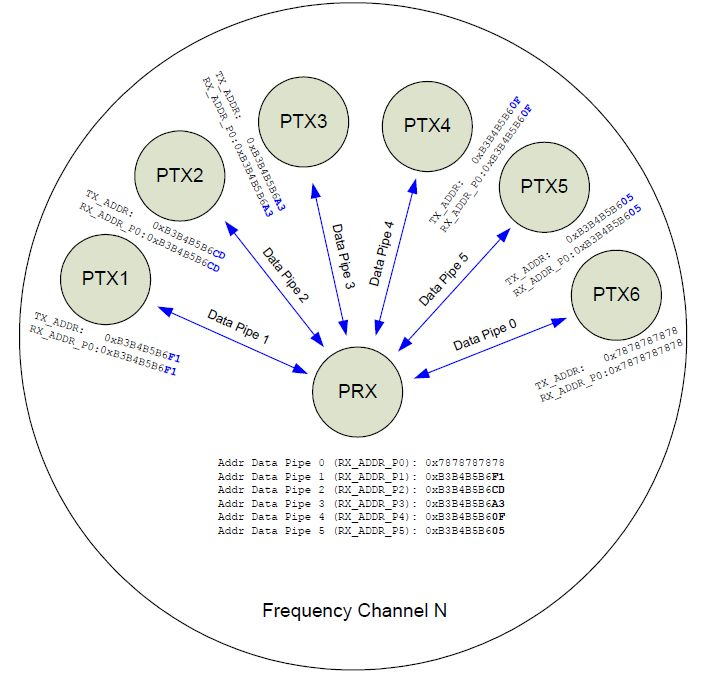
\includegraphics[width=0.4\linewidth]{Afbeeldingen/nrfMulticiever.jpg}\end{center}
	\caption{Werking van verbindingen nRF24l01. Afkomstig van \href{https://www.instructables.com/id/NRF24L01-Multiceiver-Network}{https://www.instructables.com/id/NRF24L01-Multiceiver-Network}, 18 maart 2019}
	\label{fig:nrfchannel}
\end{figure}
Hij kan tot zes kanalen tegelijk open houden die kunnen schakelen tussen een RX (ontvang) en TX (zend) stand. 
\autoref{fig:nrfchannel} laat het gebruik van adressen zien, hierin is te zien dat een adres is opgebouwd uit 5 bytes.
Dit levert een totaal op van 10782039375 ($255^{5}$) unieke adressen.
Het grote aantal zal waarschijnlijk nooit bereikt worden door de complexiteit die de topologie van een dusdanig netwerk geeft.
De modules versturen pakketten met een maximale grootte van 32 byte.


Als er gekeken wordt naar de populaire libary genaamd nRF24 dan wordt er gebruikt gemaakt van 1 byte voor het adres wat 255 unieke mogelijkheden geeft.
De samenstelling van een pakket is af te lezen in \autoref{tab:nrf} \nameref{tab:nrf}

\begin{table}[H]
	\centering
	\begin{tabular}{l|l|l|l|l|l|}
		\cline{2-6}
		& \cellcolor[HTML]{C0C0C0}FROM & \cellcolor[HTML]{C0C0C0}\begin{tabular}[c]{@{}l@{}} TO\end{tabular} & \cellcolor[HTML]{C0C0C0}FORWARD & \cellcolor[HTML]{C0C0C0}ACK & \cellcolor[HTML]{C0C0C0}PAYLOAD \\ \hline
		\multicolumn{1}{|l|}{\cellcolor[HTML]{C0C0C0}\begin{tabular}[c]{@{}l@{}}Aantal\\ Bytes\end{tabular}} & 1                          & 1                                                                               & 1                                & 1                                 & 28                                                          \\ \hline
	\end{tabular}
	\caption{NRF24 libary pakket}
	\label{tab:nrf} 
\end{table}

In deze toepassing blijft er dus ruimte over voor 28 bytes als payload wat nog steeds voldoende zou zijn voor de netwerkmodules van de drones.


\subsection{Conclusie keuze hardware: LoRa vs nRF}

Er zijn nu twee kandidaten voor het netwerk.
De LoRa PHY module die gigantische afstanden kan afleggen maar als keerzijde een langzame verbinding heeft.
Als andere kandidaat is er de nRF24l01+ een module die vele malen sneller is maar dan ook flink inlevert op het bereik ten opzichte van LoRa.

Omdat beide modules voldoen aan de gestelde eisen en in staat zijn de gewenste payload te versturen zijn ze voorgelegd aan de technisch manager van Alten Nederland.
Hij ziet een betere business case in een netwerk met een hogere dichtheid maar dan ook een hogere snelheid.
Daarom zal er in dit project gebruik gemaakt worden van de nRF24l01+.



\section{Welke routeringstechniek is geschikt voor de te gebruiken hardware?}
\label{sec:meshnetwerktechniek}

Het netwerk wordt opgebouwd door het toepassen van een meshnetwerktechniek.
Wat een meshnetwerk is wordt al toegelicht in \autoref{sec:meshnetwerkkeuze:watismesh}.
Een kenmerkend eigenschap van een meshnetwerk is het hebben van meerdere verbindingspunten per router of gateway. Dit wordt opgezet door een routeringstechniek. Er zijn verschillende technieken met elk voor en nadelen. De technieken zijn te verdelen in drie groepen: proactieve, reactief en hybride \cite{meshprotocols}. Het verschil tussen deze technieken zit hem in ontdekken van andere nodes in het netwerk. In de hierop volgende paragrafen worden deze technieken kort toegelicht. Vervolgens zal besloten worden welke van deze drie het meest geschikt is voor de te gebruiken hardware. Tenslotte zal gekeken worden binnen die groep gekozen worden welk techniek uitgewerkt wordt.

\begin{figure}[H]
	\begin{center}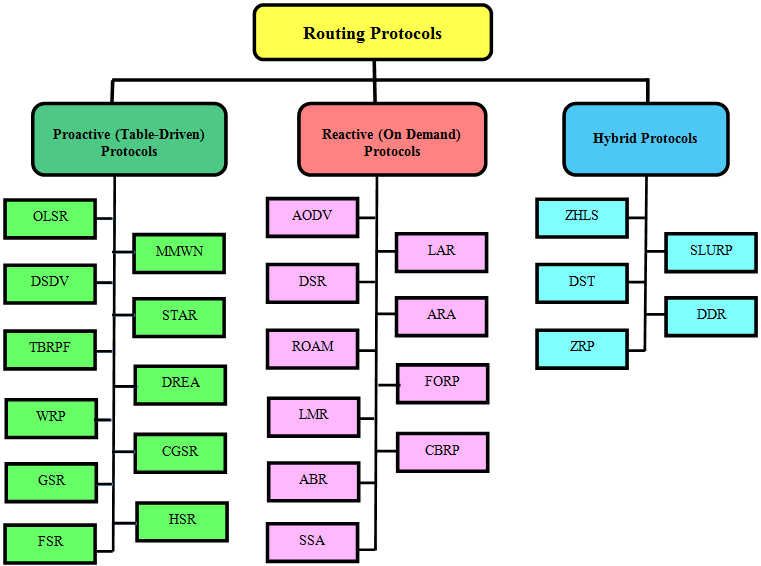
\includegraphics[width=0.6\linewidth]{Afbeeldingen/meshprotocollen.png}\end{center}
	\caption{Bestaande routeringsprotocollen. Afkomstig van \protect\cite{meshprotocols}}
	\label{fig:meshprotcollen}
\end{figure}

\subsection{Proactieve routeringstechniek}
\label{sec:meshnetwerktechniek:proactief}

Een proactief protocol is een protocol die zelf constant bezig is met het zoeken naar nieuwe punten in het netwerk.
De nodes zorgen dat veranderingen meteen kenbaar gemaakt worden aan andere punten in het netwerk. 
Dit zorgt ervoor dat het netwerk een zelf herstellend vermogen heeft en geschikt is voor het opsporen van fouten in het netwerk.
Het protocol is geschikt voor situaties waar de posities van nodes zelden tot nooit veranderen. 
In situaties waar paden vaak veranderen door het veranderen van node posities zal het protocol veel meer bandbreedte vragen van het netwerk. 

\begin{figure}[H]
	\begin{center}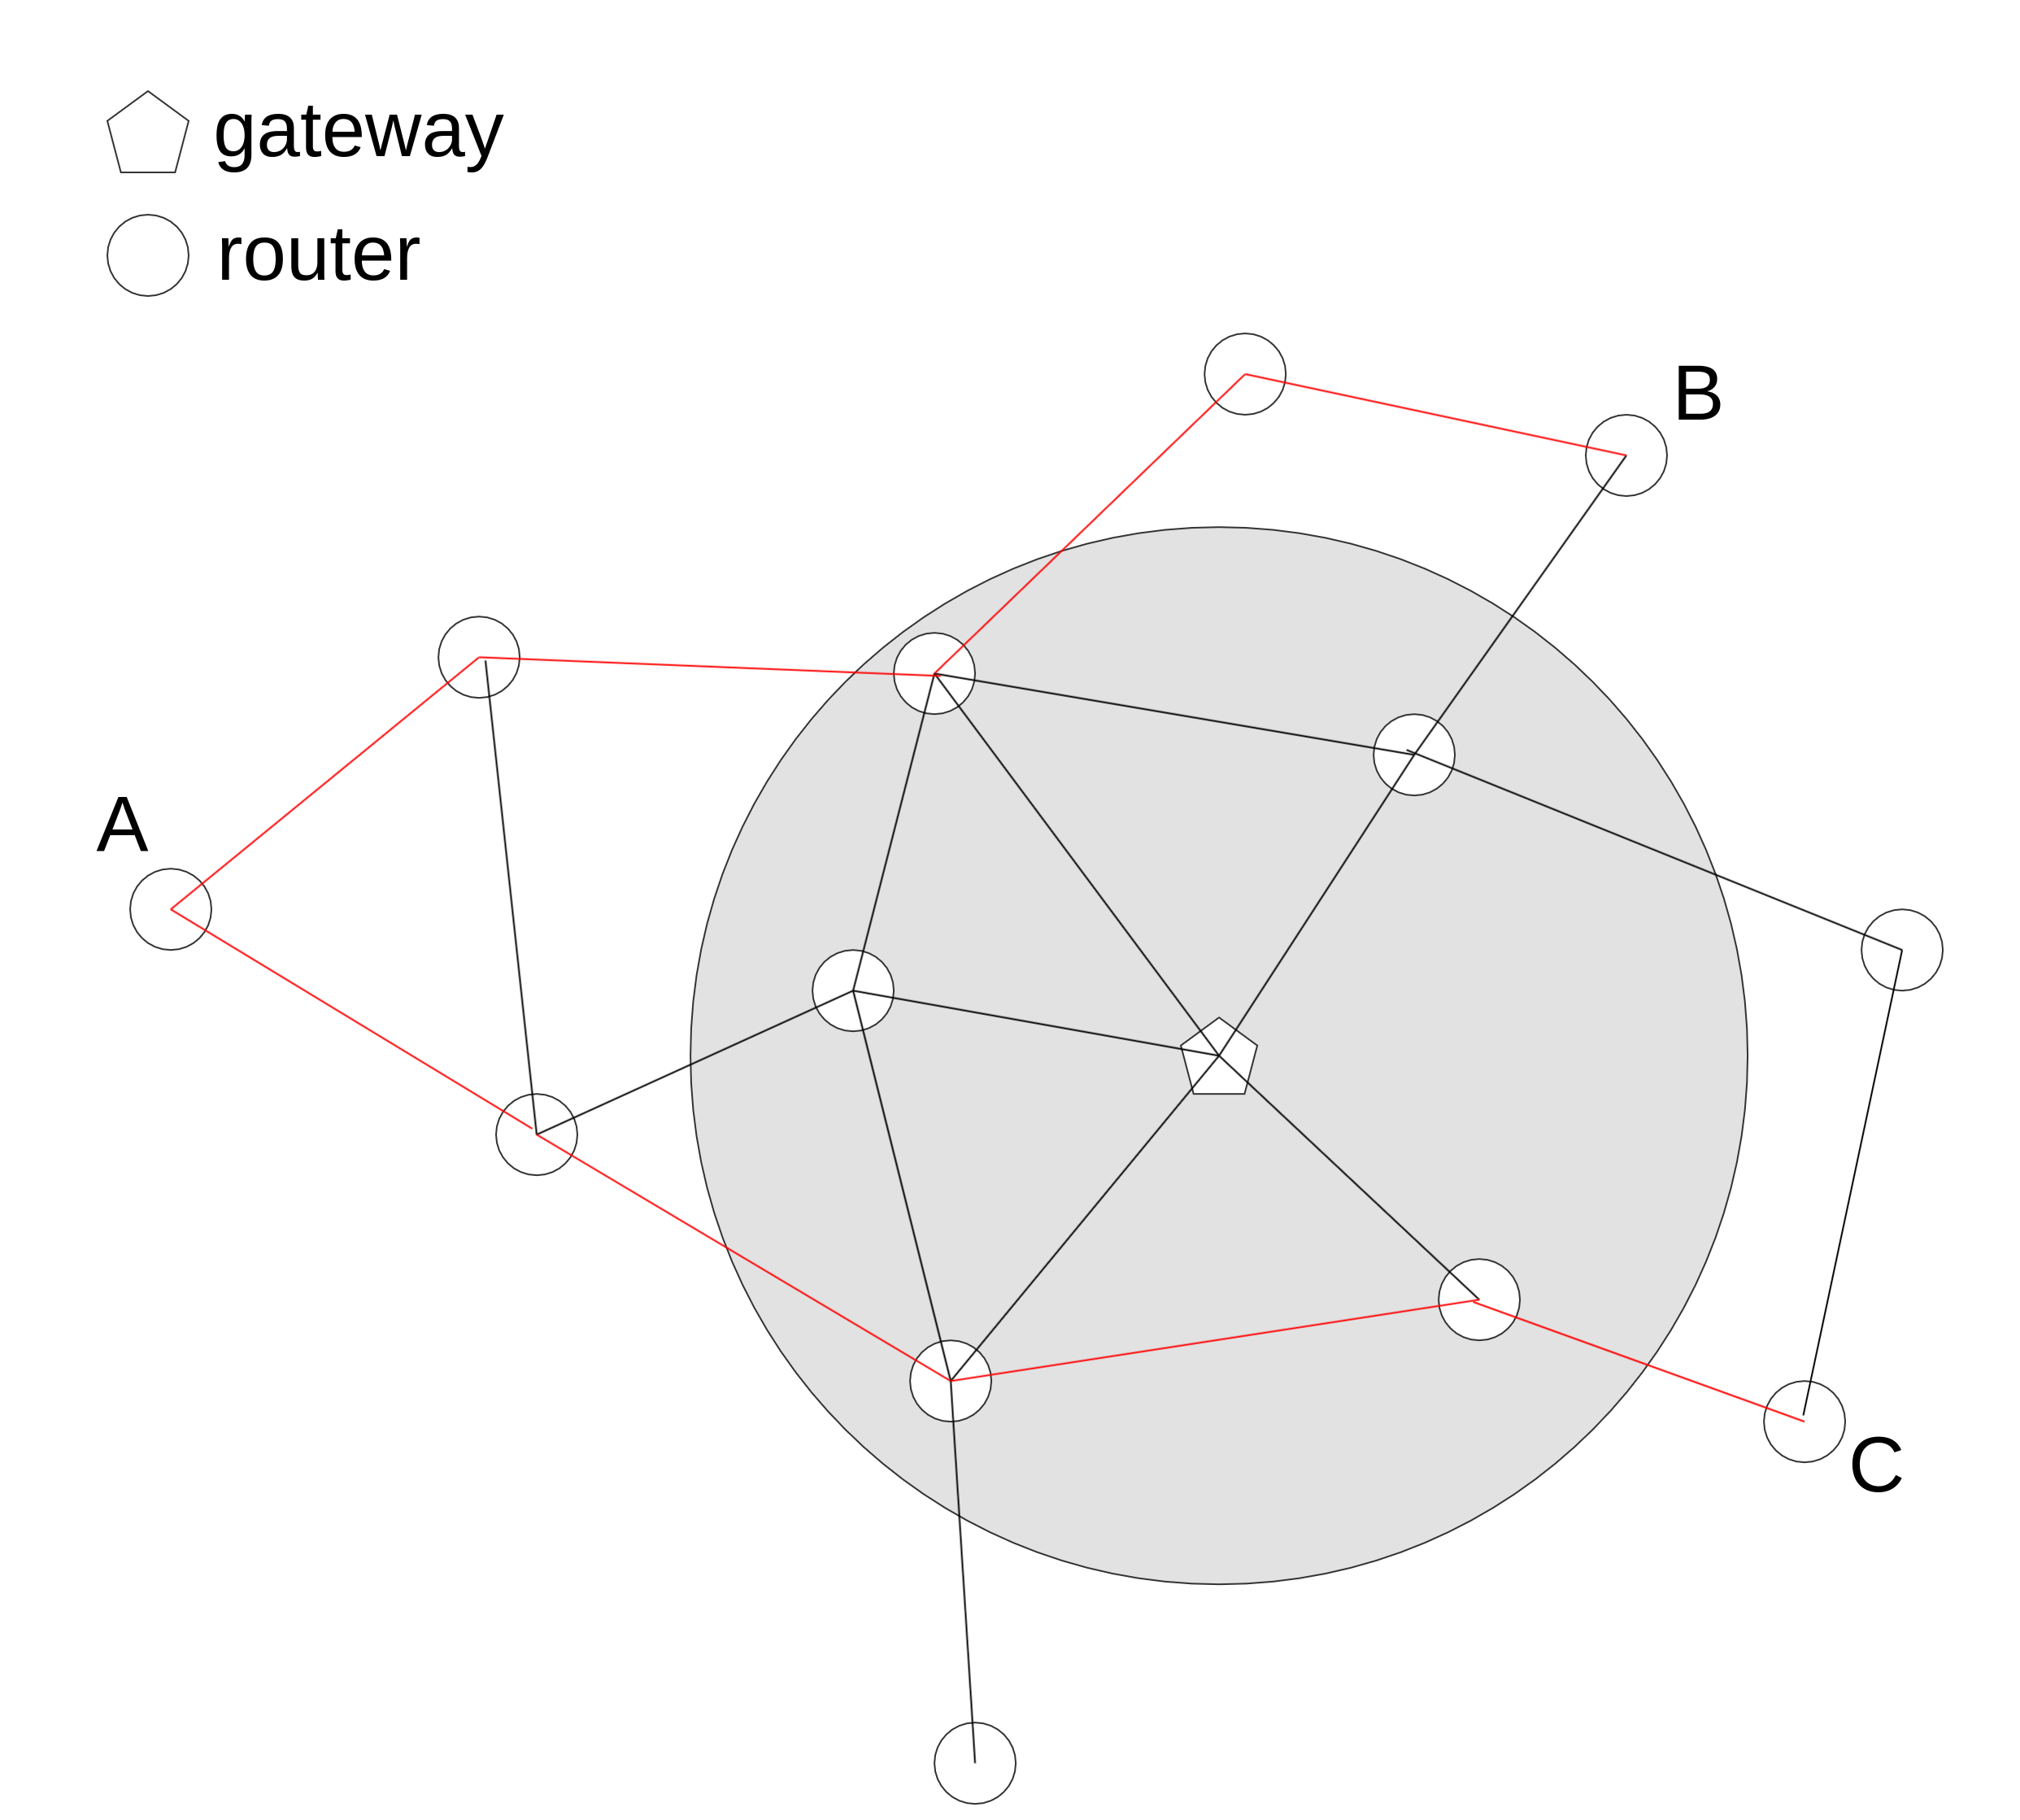
\includegraphics[width=0.45\linewidth]{Afbeeldingen/proactive.png}\end{center}
	\caption{Voorbeeld proactieve routeringstechniek.}
	\label{fig:proactief}
\end{figure}

In \autoref{fig:proactief} wordt een voorbeeld getoond waar punt A een bericht wil versturen naar punt B en C. 
Punt A is op de hoogte van alle routes in het netwerk net als de andere punten in het netwerk dat zijn.
In de huidige situatie zijn er 21 verbindingen in het netwerk tussen de nodes.
Er zijn 14 punten aanwezig in het netwerk minimaal zullen er dus voor het op de hoogte brengen van bestaande verbindingen 294 ($14 \times 21$) berichten rondgestuurd moeten worden. 

Vervolgens kan er een pad gemaakt worden waarover een bericht verstuurd kan worden.
Dit voorbeeld laat goed zien dat deze routingstechniek zijn voordeel haalt wanneer de nodes stil blijven staan omdat er dan niet opnieuw berichten verstuurd hoeven te worden. 
 
\subsection{Reactieve routeringstechniek}
\label{sec:meshnetwerktechniek:reactieve}

Een reactieve routeringstechniek is een methode waarbij de nodes geen routes opslaan maar op aanvraag routes opbouwen. 
Dit scheelt in het gebruik van geheugen en het heeft minder berichten bij het initialiseren van het netwerk. Daarentegen kost het deze techniek meer tijd om een bericht te versturen omdat er voordat er een bericht verstuurd kan worden eerst een route opgebouwd moet worden.

\begin{figure}[H]
	\begin{center}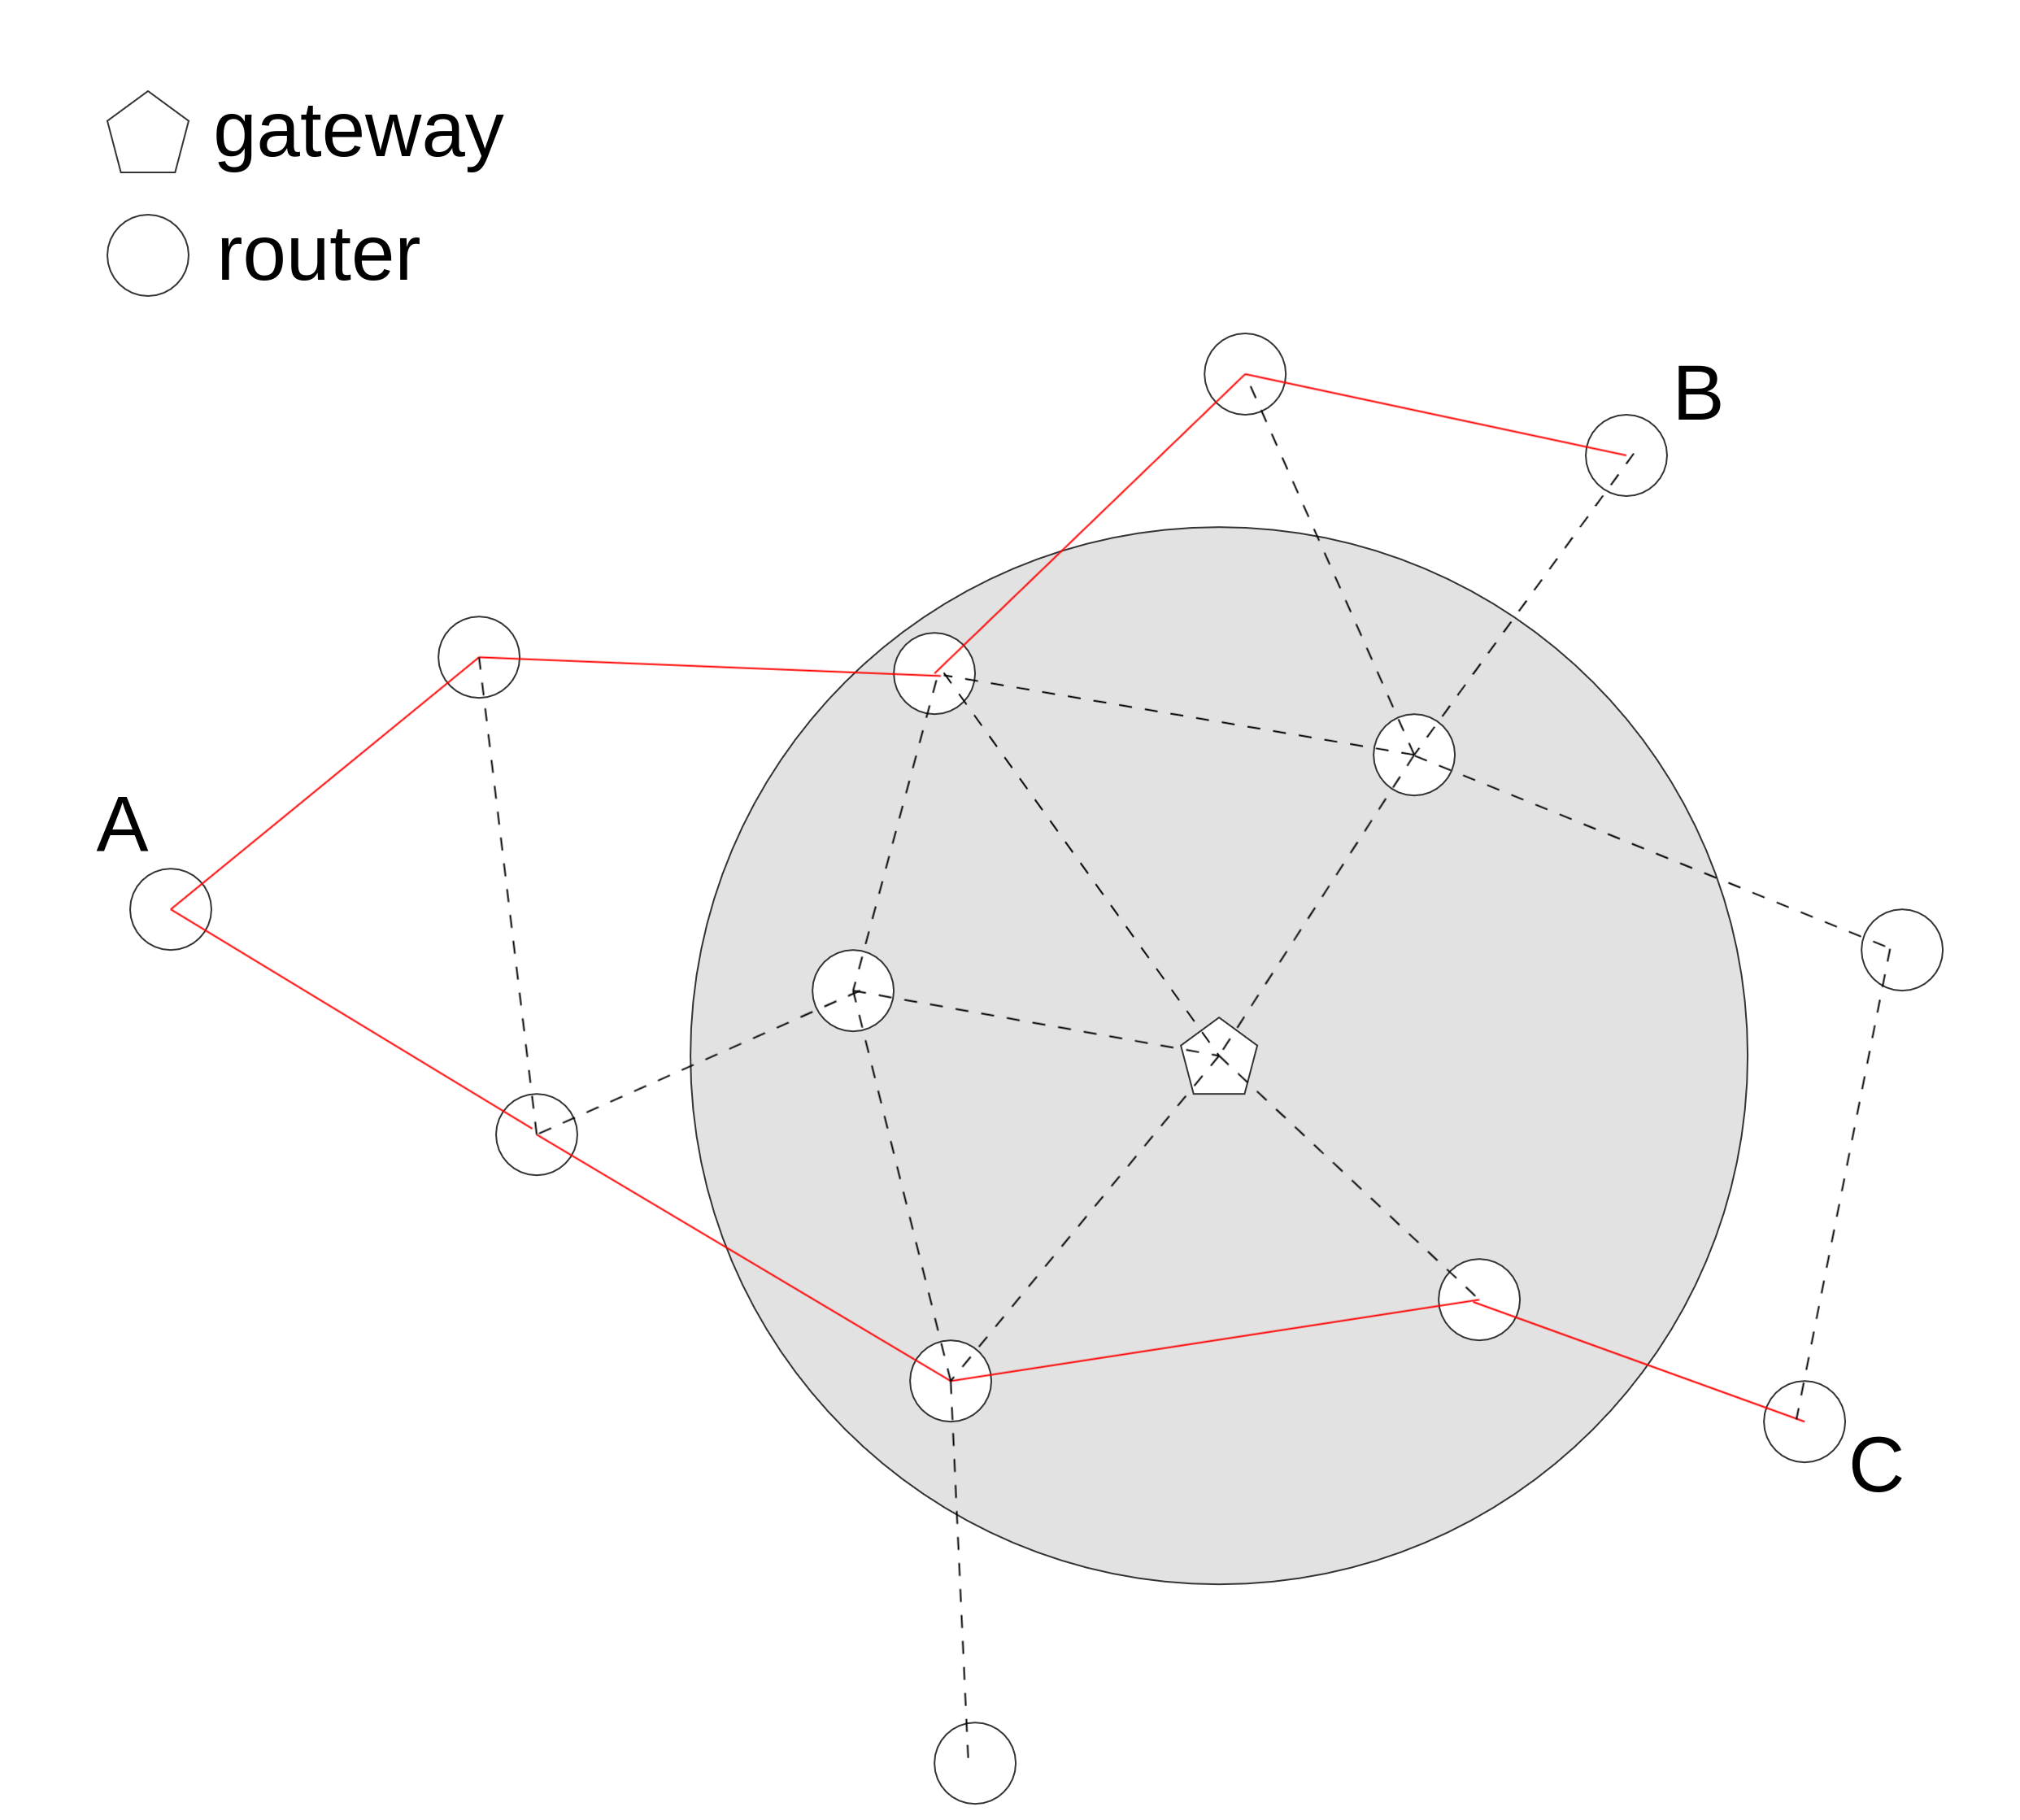
\includegraphics[width=0.45\linewidth]{Afbeeldingen/reactive.png}\end{center}
	\caption{Voorbeeld proactieve routeringstechniek.}
	\label{fig:reactief}
\end{figure}

\autoref{fig:reactief} laat een voorbeeld zien waarin er gebruik gemaakt wordt van een reactieve routeringstechniek.
Er zal in dit voorbeeld voordat een route gezocht wordt er een route gemaakt moeten worden tussen de twee punten.
Vervolgens als deze route gevonden is zal er een bericht hierover gestuurd worden. 
Deze route wordt tijdelijke opgeslagen tot de node klaar is met het versturen van zijn data.

\subsection{Hybride routeringstechniek}
\label{sec:meshnetwerktechniek:hybride}
Een hybride routeringstechniek is een techniek die een proactieve en reactieve techniek deels combineert om zo ongewenste nadelen te elimineren van elkaar. 

\begin{figure}[H]
	\begin{center}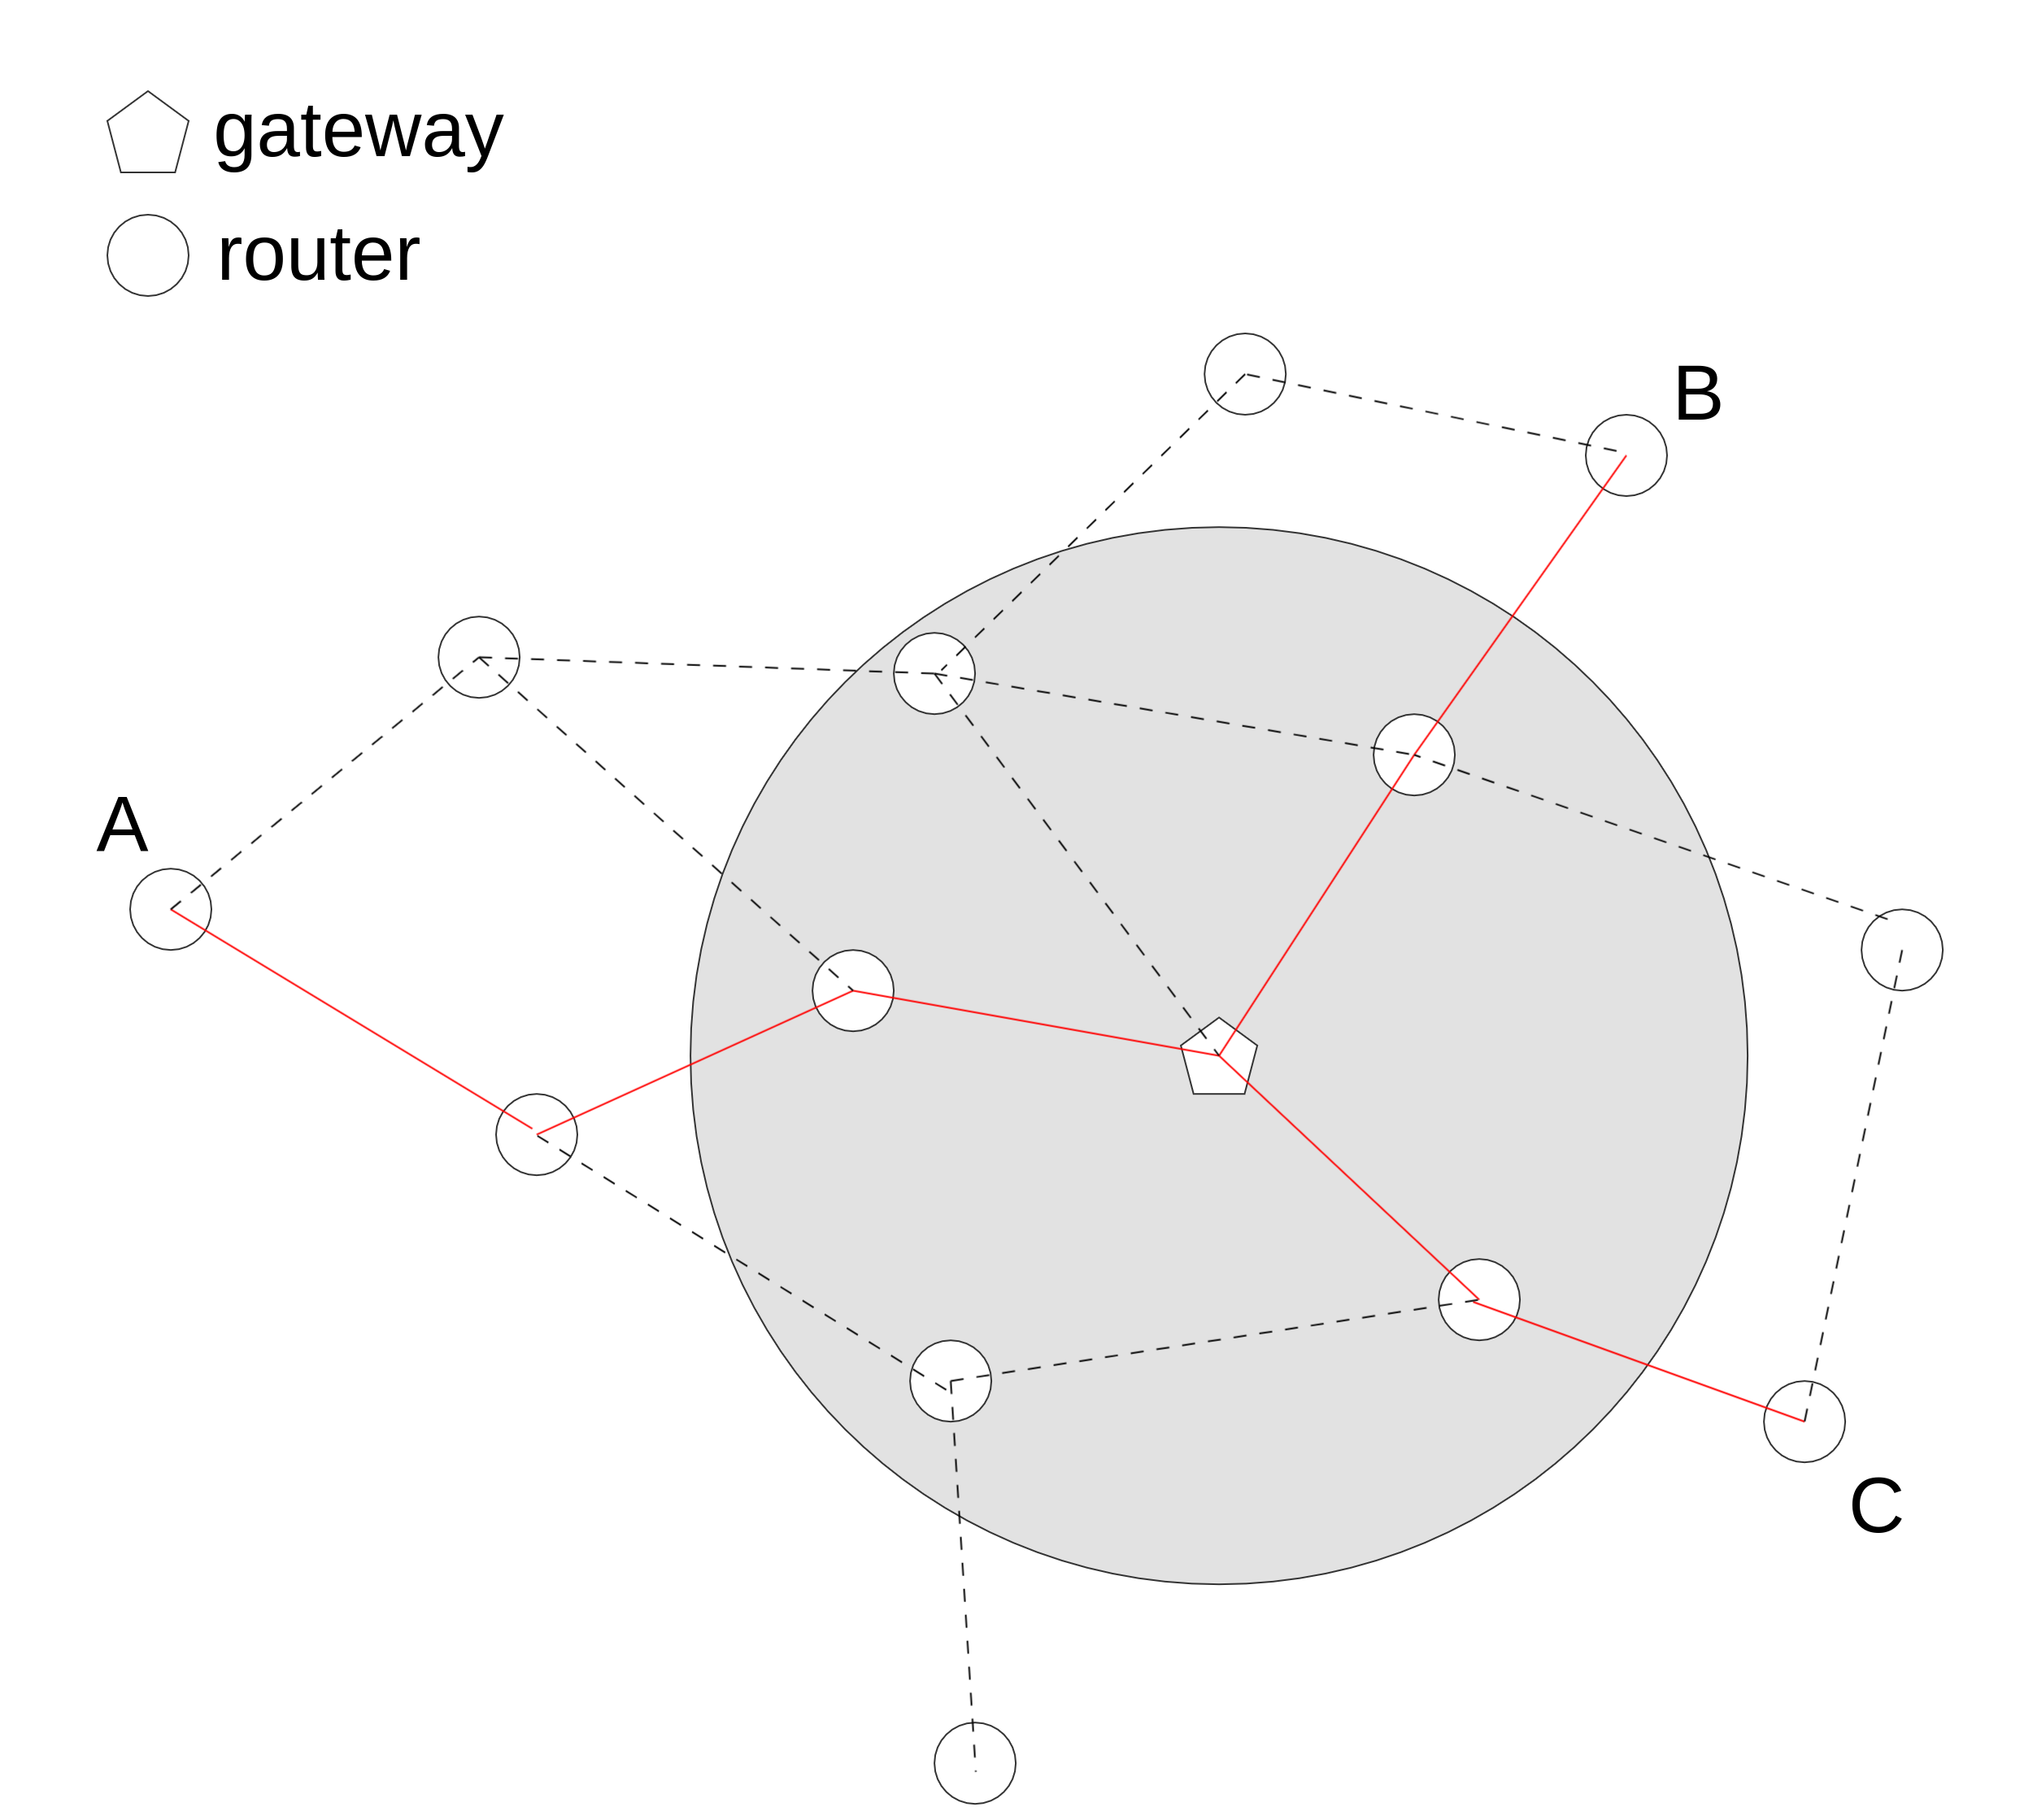
\includegraphics[width=0.45\linewidth]{Afbeeldingen/hybride.png}\end{center}
	\caption{Voorbeeld hybride routeringstechniek.}
	\label{fig:hybride}
\end{figure}

In dit voorbeeld is een hybride routeringstechniek uitgewerkt er zijn veel meer varianten aanwezig het voorbeeld is om te laten zien hoe reactief en proactief geactiveerd wordt.
In deze situatie is de gateway voorzien van een proactief protocol waardoor het alle routes kent. 
De routers hoeven daardoor alleen een route te bereken naar een gateway toe.   
  
\subsection{Conclusie}
\label{sec:meshnetwerktechniek:Conlusie}
Het dronenetwerk is een netwerk die vaak te maken zal hebben met verplaatsingen.
De hele eigenschap om autonoom nodes te kunnen verplaatsen is zelf de aanleiding van het project.
Daardoor vallen een proactieve routeringstechnieken af. 
Toch is de tegenhanger reactieve routering ook geen ideale oplossing.
Het niet opslaan van routes maakt het versturen van berichten sloom en er is geheugen aanwezig op de microcontroller voor het opslaan van routes. 

Daarom is de conclusie om een zelf een hybride variant te maken van het reactieve Lightweight Mobile Routing(LMR) protocol.
Dit protocol wordt gebruikt omdat het een protocol is die een hop routeringstechniek gebruikt waardoor de payload klein blijft.
De techniek is niet afhankelijk van een gateway en nodes hoeven alleen te bewust te zijn van de buren en met wie die buren verbonden zijn.
Het protocol hoeft alleen maar aangepast te worden zodat routes opgeslagen blijven.
Doordat deze techniek geen routes hoeft op te slaan van het volledige netwerk  maar allen die van hun aangesloten buren en hun aangesloten punten zullen er geen grote routeringstabellen gecreëerd worden.


\section{Wat is minimaal benodigd in een simulatie om abstracte drone te representeren?}
\label{sec:dronekeuze}

In \autoref{sec:welkesim} is geconcludeerd dat als simulatie software ROS melodic met Gazebo9 wordt gebruikt.
Hierin kwam naar voren dat niet elke drone package gebruikt kan worden doordat ze specifiek gemaakt zijn voor de versie van ROS.
Omdat het project de focus heeft op de werking van netwerkmodules voldoet een abstracte versie van een drone.
Zo hoeft deze bijvoorbeeld op dit moment nog niet realistisch te vliegen.

Daarom is besloten dat de drone het volgende moet kunnen in de simulatie:

\begin{itemize}
	\item Een drone moet verticaal kunnen opstijgen.
	\item Een drone moet verticaal kunnen landen.
	\item Een drone moet zich kunnen voortbewegen.
	\item Een drone verplaatsing begint altijd met opstijgen en eindigt altijd met een landing.
	\item Een drone moet voorzien zijn van module die een locatie kan teruggeven. 
	\item Een drone moet mag een basisvorm gebruiken om zich zichtbaar te maken in de simulatie
\end{itemize}


\chapter{Oplossingsrichtingen}

\begin{itemize}
\item Beschrijf je hoe jouw oplossingsrichting de hoofdvraag beantwoord?
\item Beschrijft de oplossingsrichting de mogelijkheden?
\item Staat hier "Veld" vermeldt van de methodekaart van de HAN?
\end{itemize}
\hrule



\chapter{Experimenten}
\label{experimenten}

\begin{itemize}
	\item Beschrijft waarom dit experiment van belang is.
	\item Voldoet de code van het experiment aan de opgestelde eisen?
	\item Voldoet het programma aan de opgestelde QoS?
	\item Is gedocumenteerd waarom het programma voldoet aan de opgestelde eisen?
	\item Is gedocumenteerd waarom het programma voldoet aan de opgestelde QoS?
\end{itemize}
\hrule

\section{Hoe gedraagt een node uit het mesh netwerk zich bij slecht of geen bereik?}
\label{experimenten:slechtofgeenbereik}

%TODO snel definiëren
\section{Wat kan er toegevoegd worden aan de communicatie van de netwerkmodule om snel achter uitval te komen?}
\label{experimenten:snelachteruitval}

\chapter{Conclusie}

\label{chapter:conclusie}
Conclusie uit resultaten. Herhaal en beantwoord de hoofdvraag.
\begin{itemize}
\item Trek een conclusie uit de resultaten van de deelvragen.
\item Wordt de hoofdvraag beantwoord?
\item Wat beveel je aan?
\end{itemize}
\hrule


\bibliographystyle{apacite}
\bibliography{bilbliography.bib}

\clearpage
\appendix
\chapter{Schets voor casus drone netwerk}
 \label{app:schetsNetwerk}
\begin{figure}[H]
	\begin{center}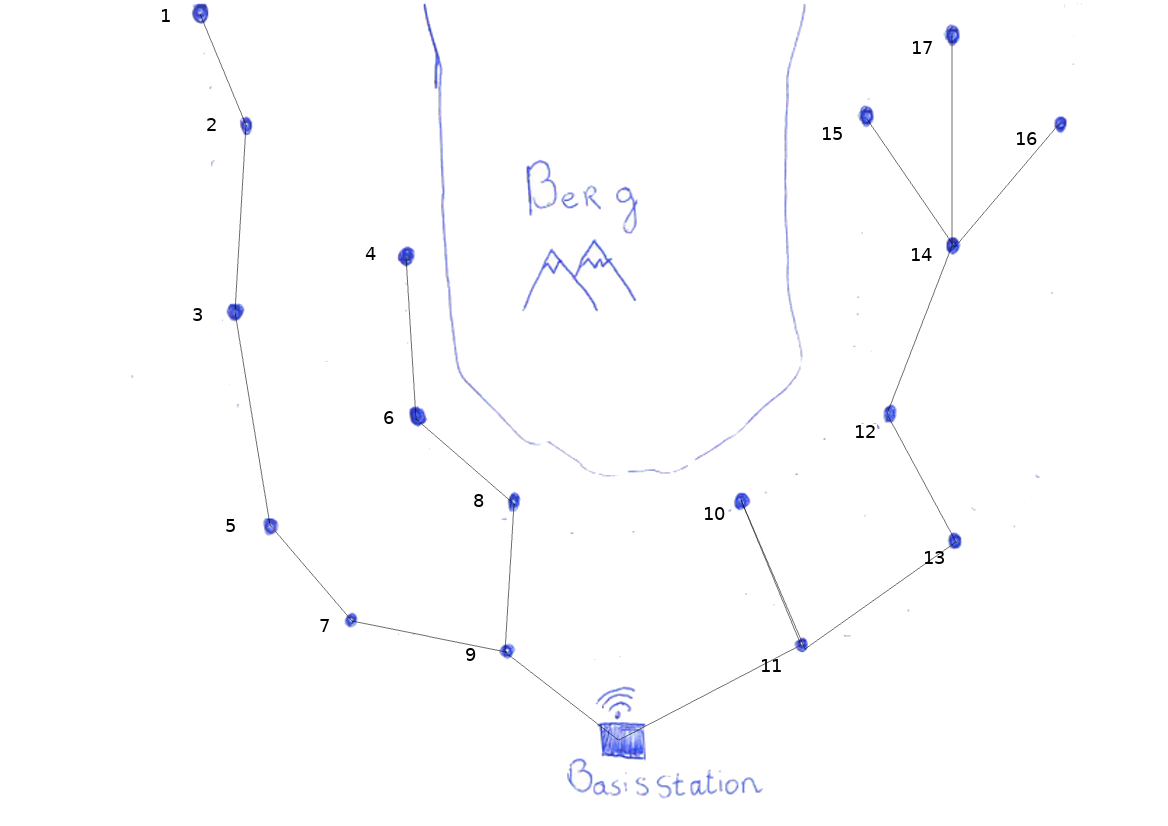
\includegraphics[width=\linewidth]{schetsNetwerk}\end{center}
	\caption{Schets van casus netwerk}
	\label{fig:schetsNetwerk}
\end{figure}

\end{document}